  %% A novel ranking-based
%% inference was used to establish that trade was indeed a driving factor in the
%% rapid spread of the pest in this region.
%% In general, modeling the multi-pathway dispersal of pests such as \tuta{}
%% is a challenging task due to inadequate understanding of the complex
%% interconnected food system. To add to the
%% problem, most countries ended up not being prepared for the infestation,
%% either due to lack of awareness of the pest or the sheer speed of invasion.
%% Absence of quality incidence records makes callibration and validation
%% hard. Some of these problems were highlighted in the modeling
%% effort by 

%% In recent years, there has been a thrust towards integrated modeling
%% approaches to understand invasive species dynamics.%%     \textbf{Interventions.} The effect of
%% reducing outflows from major production regions is shown for Class~B
%% models. These are representative results for Philippines. Plots for other
%% countries are in Figure~\ref{S:fig:intervene}. In the simulations, a high
%% production region (Northern Mindanao) was seeded. (a)~\textbf{Without
%% intervention.} Simulations indicate that for the given initial conditions,
%% there is a high chance that all major production areas of Philippines will
%% be affected within 24 months.  The colors indicate the time interval at
%% which there is at least a 50\% chance that a location will be infected.
%% (b)~\textbf{With market level intervention.} The spread without the
%% influence of long-distance flows from localities corresponding to high
%% production areas (Northern Mindanao and Central Luzon). We observe a delay
%% of more than two years in the introduction to the northern part due to this
%% intervention.  (c)~\textbf{Spread with respect to origin of infection.}
%% We compare the effect of reducing the long-distance flow the
%% above-mentioned regions by 50\% and 100\%. The results shown correspond to
%% all Class~B instances with Moore range~$\mooreRange=1$. \label{fig:intervene}}
%% Under the assumption that appropriate control
%% measures are taken, we reduce the incoming and outgoing edge weights
%% by~$50\%$ of their original value. The resulting model was compared with
%% the case where no action is taken (Section~\ref{sec:predict}).
%% 
%% Farm-level \aacomment{not sure about this}
%% \begin{itemize}
%%     \item suitability threshold is varied
%%     \item Scenario 1 where for all cells it is done
%%     \item Scenario 2 where for it is done in key tomato growing areas
%%     \item Scenario 3 where it is done only near localities
%% \end{itemize}
%% 
%% Market-level
%% \begin{itemize}
%%     \item Scenario 1: we identify localities which are hubs (lots of
%%     outflow) and reduce their flow.
%% \end{itemize}
%% %%
%% \begin{figure}[ht]
%%     \centering
%%     \begin{subfigure}[b]{.47\textwidth}
%%         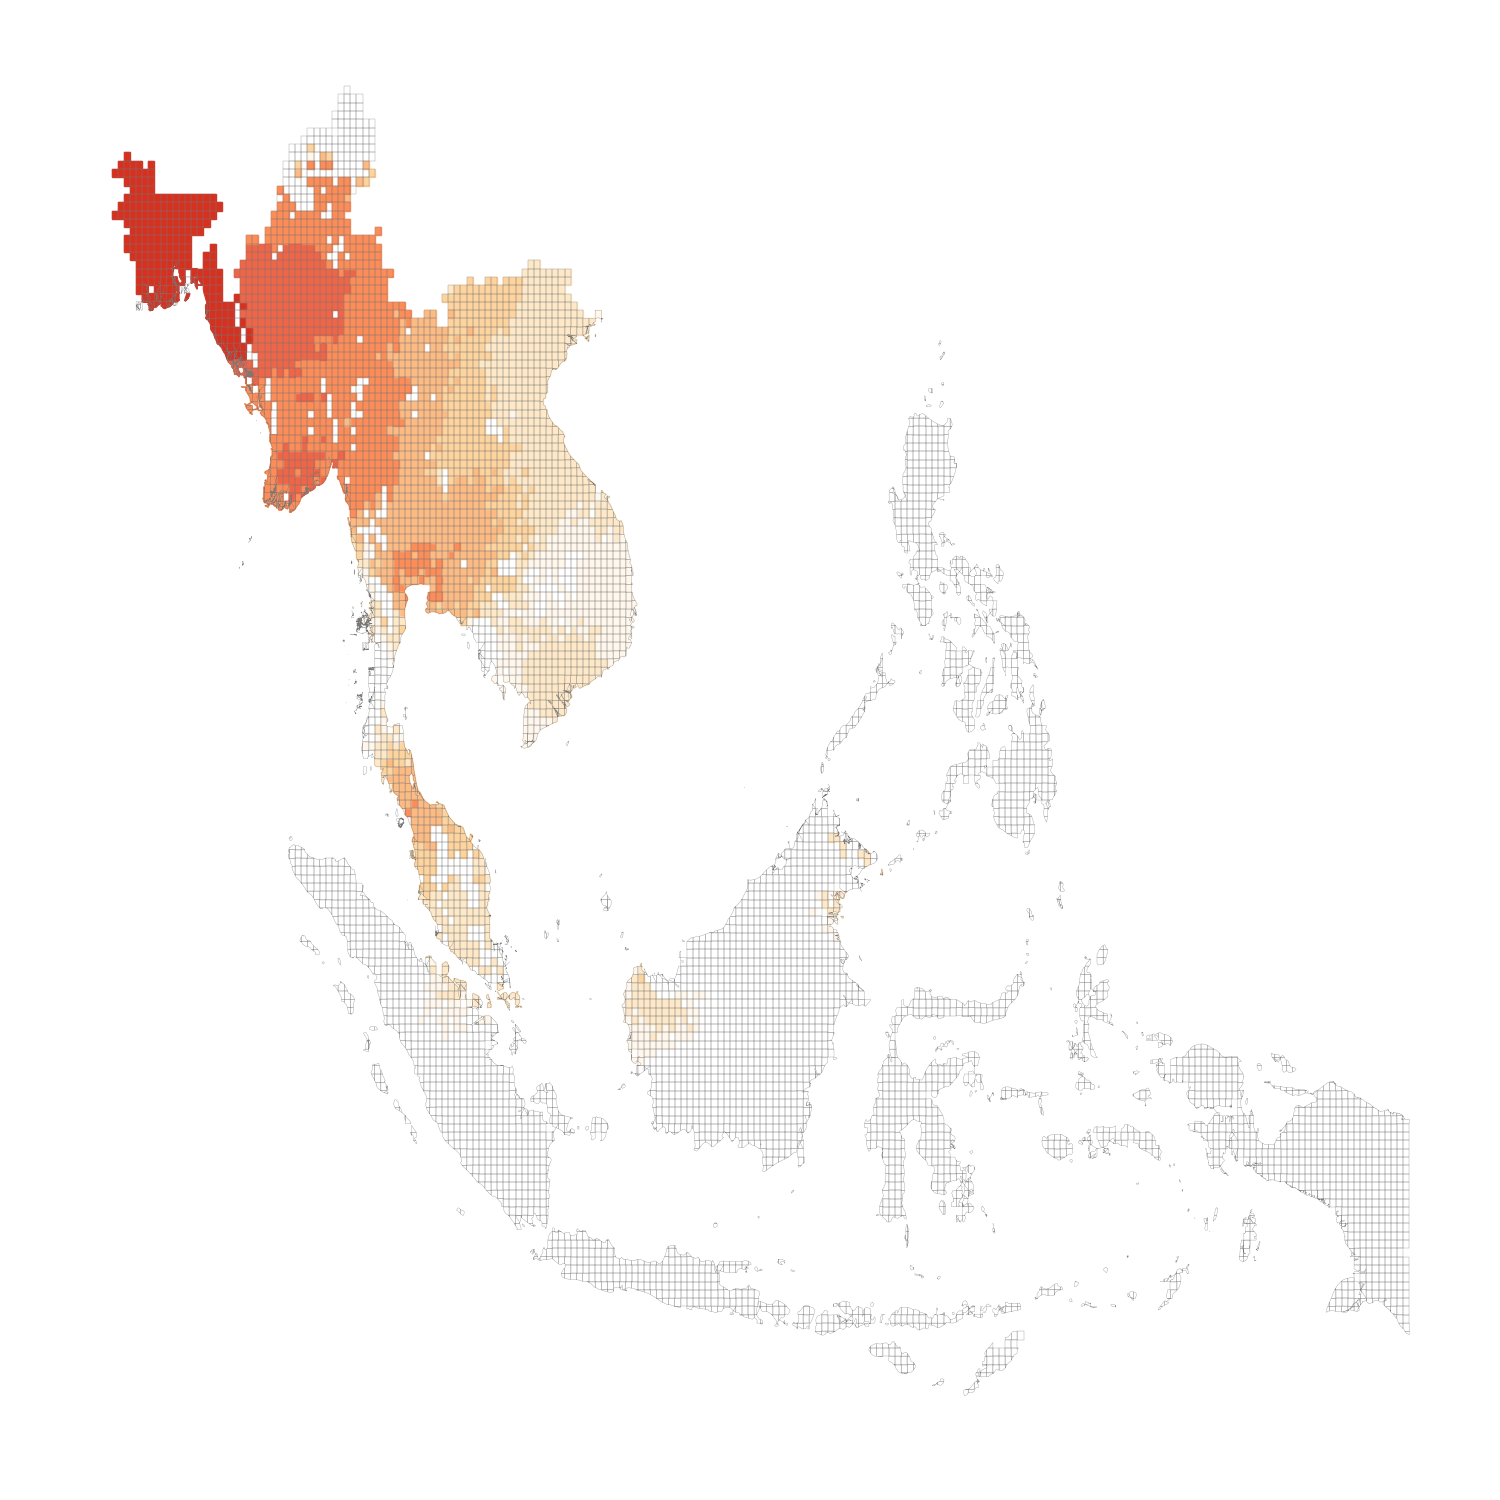
\includegraphics[width=\textwidth]{figs/spread_farm_level_interventions.png}
%%     \caption{\label{fig:spreadFarmLevel}}
%%     \end{subfigure}
%%     \begin{subfigure}[b]{.47\textwidth}
%%     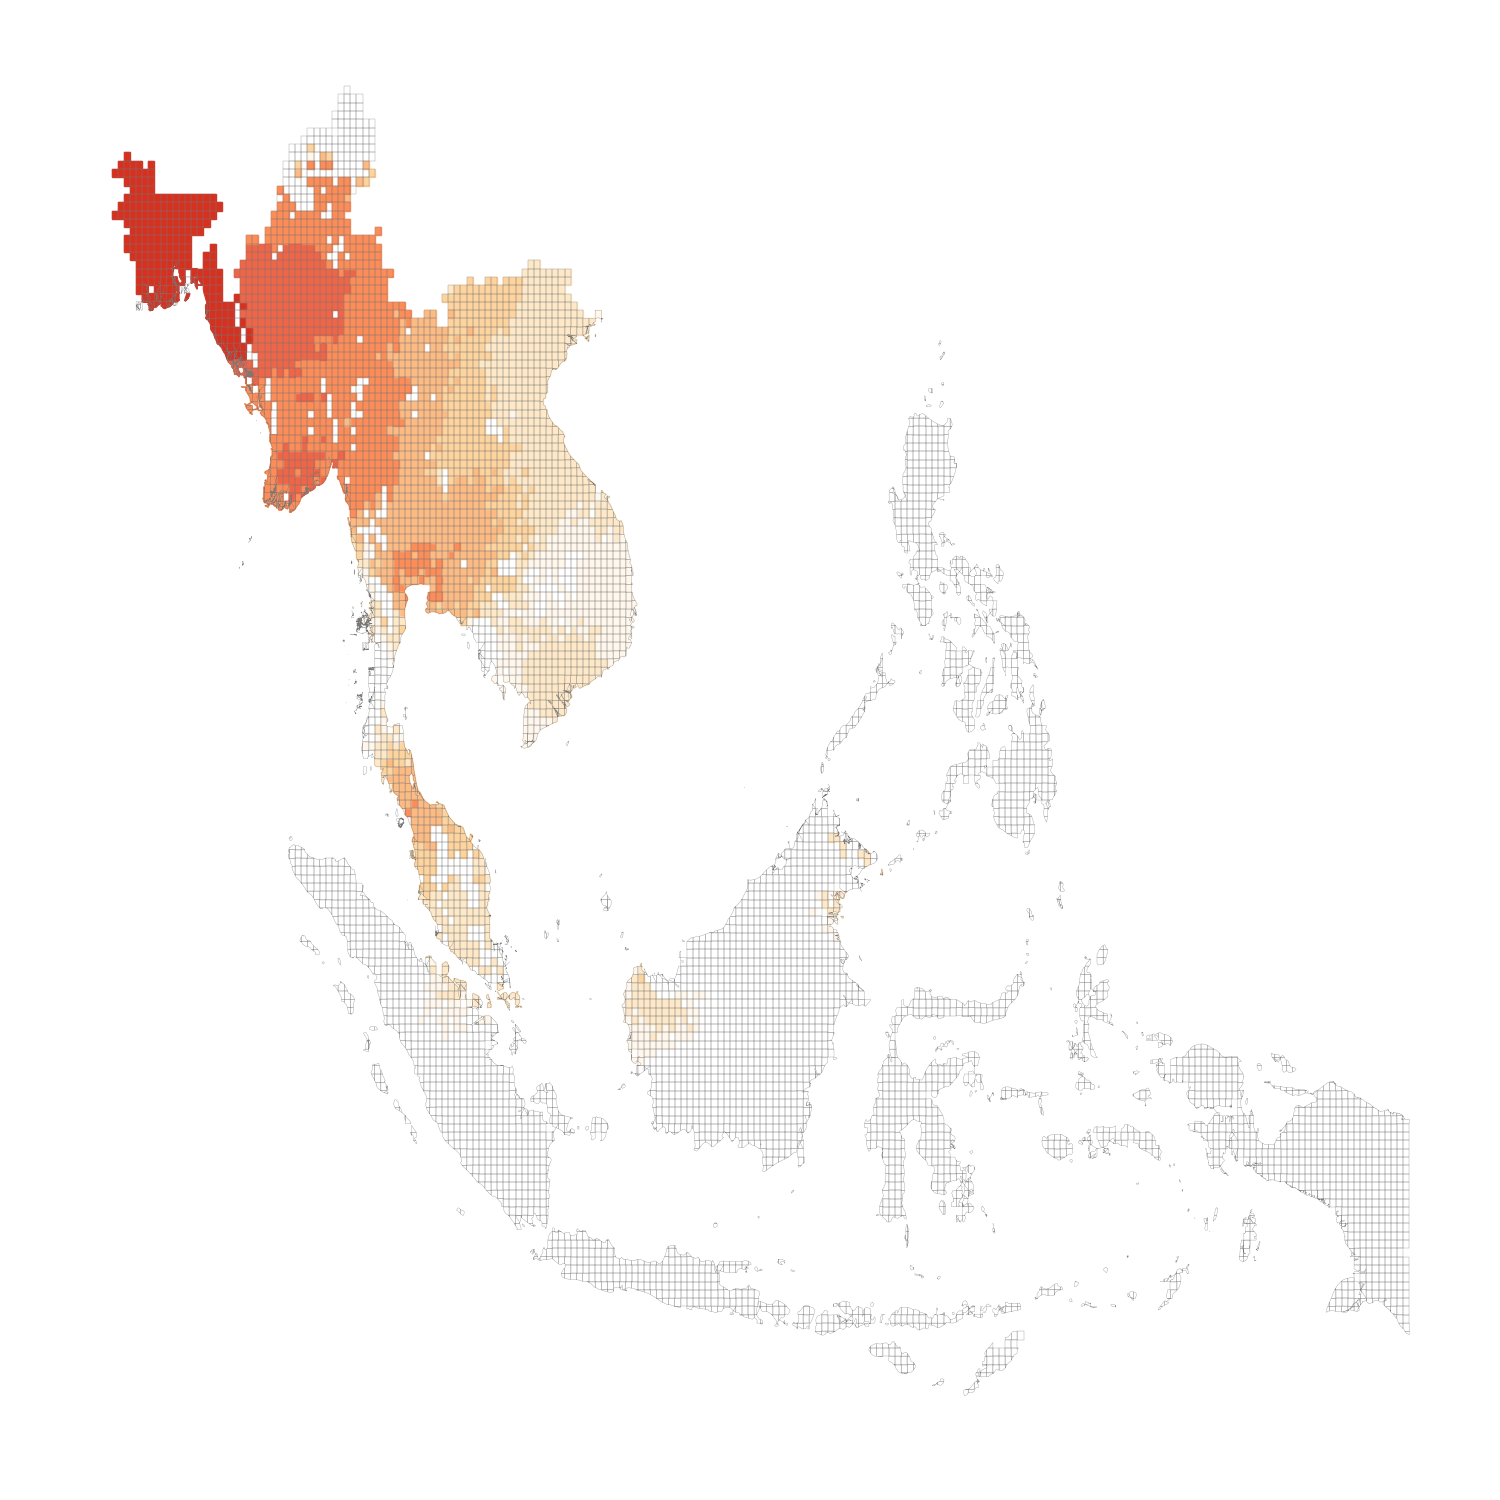
\includegraphics[width=\textwidth]{figs/spread_market_level_interventions.png}
%%     \caption{\label{fig:spreadMarketLevel}}
%%     \end{subfigure}
%%     \caption{Effect of interventions}
%% \end{figure}
%% Given the importance of the long-distance human-mediated pathway, we
%% studied the effect of controlling this pathway in mitigating the spread.
%% Monitoring localities by setting up pheromone traps in production areas and
%% markets, and quarantining affected areas is one way to accomplish this.
%%
%% According to Figure, the assumptions of linearity, normality,
%% and homogeneity tended to be fairly met. For the assumption of independent
%% observation, however, the product rates are not independent each other
%% within region, so caution needs when interpreting the results.


%% To predict seasonal production, we used regional quarterly tomato and
%% eggplant production data that was available for Philippines~\cite{psa} (16
%% regions), precipitation and elevation data at the cell level. For each
%% region, we obtained the product rate by normalizing quarterly production
%% values with respect to maximum value among these. We used production rate
%% instead of production values since there are several factors that determine
%% a region's production: climate, vegetable preference, demand, etc.
%% Therefore, it may not be meaningful to compare production across regions.
%% We conducted a linear regression with the product rate as a dependent
%% variable and precipitation and elevation as independent variables
%% (SPSS~24.0). Since the dependent variable was highly skewed, we used a
%% log-transformation. To control elevation, we classified the elevations into
%% two groups, high and low, using $k$-means clustering (SPSS~24.0). Due to
%% the small sample size, we excluded the samples in the high-elevation group
%% and conducted a linear regression analysis for the group of low
%% elevation~($< 235$). The total 56 samples in the group showed negatively
%% strong correlation between precipitation and logarithm of product rate
%% ($r=-0.734$). 
%% For most countries, only qualitative information on seasonal production is
%% available making validation near impossible.  However, we observed that for
%% the entire region seasonal production was strongly tied to rainfall; during
%% the wet season, the amount of production is considerably less compared to
%% the dry season.
%% 
%% The regression results showed that the precipitation was a statistically
%% significant predictor ($p <0.001$, $R^2=0.54$) in Table 1. For assumptions
%% of linear regression According to Figure 1, the assumptions of linearity,
%% normality, and homogeneity tended to be fairly met. For the assumption of
%% independent observation, however, the product rates are not independent
%% each other within region, so caution needs when interpreting the results.
 More details of the
CART analysis is presented in Section~\ref{S:sec:cart}.  

DOAS
============================================================
VN starting cells not true to radial spread


Random Forest (RF), proposed by Breiman(2001), is a nonparametric ensemble learning method for classification and regression. This method overcomes decision trees’ problem of overfitting by constructing a multitude of decision trees. In order to allow chances to multiple strong predictors to split the trees, each tree uses only a subset of the predictors. In regression, RF predicts the response variable by averaging the predicted values from all trees. Overall, RF provides more advantages over other decision trees such as CART and Bagging, especially for accuracy and robustness.

%% .  the start
%% time step of simulation plays an important role (Figure~\ref{fig:rfShort})
%% as the spread pattern is mostly radial.
%% This is mainly because the spread pattern is radial in turn is
%% dictated by scaling factors $\asd$ and $\afm$, and start month for the
%% simulation. The gravity model parameters $\beta$ and $\kappa$ do not
%% influence this model as there is no long-distance spread. We also note that
%% the monthly production template (uniform or seasonal) does not affect the
%% spread behavior. This is mainly because the values of short-distance
%% scaling factors~$\asd$ or (and)~$\afm$ are relatively high to negate the
%% effect of heterogeneity in monthly production.
%% 
%% For the remaining ranges of~$(\mooreRange,\ell)$, we observe a richer set of
%% emergent behaviors. While for very high values of~$\ald$ and~$\afm$, we
%% again see Class~A spread pattern, Class~B dominates and is strongly
%% influenced by monthly production template, \jmcomment{and?} start month. While~$\beta$ is a
%% significant factor in the spread, the outcome is not highly sensitive
%% to~$\kappa$.


%% Our analysis strongly indicates that both short distance spread and trade
%% are important pathways in the spread dynamics. For the parameter set with
%% the best fit, the similarity was close to~$6$, i.e., on an average,
%% simulation output matched six out of eight locations.   This is in some sense
%% expected due to long distance jumps facilitated by human-assisted spread.
%% It also means that \tuta{} can achieve the same (or greater) range
%% expansion with considerably less flying capacity and population growth.

%% While our results highlight the role of human-mediated spread, it is
%% possible that this pathway is more important for the spread than it
%% appears.  First of all, vegetable production data for Bangladesh~\cite{spam}
%% indicates that almost all cells have non-zero production of hosts of
%% \tuta{}. Therefore, there is a contiguous landscape of suitable areas for
%% the pest to spread naturally. But in general this may not be the case; the
%% only way two locations can be connected is by trade or travel pathways. One
%% obvious example is two land masses separated by sea.  

%%
%%\paragraph{Sensitivity analysis.} 
%%We assessed the role of the model
%%parameters (Table~\ref{tab:parameters}) by restricting our attention.
%%\begin{itemize}
%%    \item machine learning surrogates
%%    \item CART something, default settings
%%\item If we focus on all
%%instances of parameters for which similarity is greater than~$12$ ($75\%$
%%match),
%%\end{itemize}
%%
%%

%% In the second phase,
%% we applied the select models from the previous phase to the rest of the
%% region to study how various conditions affect the nature and rate of
%% spread: different pest introduction scenarios, seasonality of production
%% and trade, and interventions or the lack thereof.
%% 
%% re
Therefore, the maximum possible value
of~$\similarity$ is~$8$ (exact match with ground truth) and minimum is~$0$.

%%
%% Each cell~$v$ has the following time varying attributes: \aacomment{these
%% are not necessary: NDVI~$\veg(v,t)$,
%% temperature~$\temp(v,t)$,} monthly production of preferred host crops and
%% consumption~$\consume(v,t)$, where~$t$ corresponds to a month.
%% \aacomment{This should get into Tonnang discussion: Since NDVI
%% data is available at a much finer resolution (see Table~\ref{tab:data}),
%% for each cell, we assign the maximum of the NDVI data points that fall in
%% this cell for that month.} For production, we consider the following
%% vegetables: tomato, potato, eggplant in metric tonnes (see
%% Section~\ref{sec:biology} on choice of host crops). Annual country-level
%% production data (in volume) is spatially disaggregated using SPAM data
%% on spatial distribution of vegetable production. \aacomment{needs
%% explanation. statistical analysis should come here}. Further, for each cell,
%% this production was distributed temporally-- one value for each month of
%% the year. We observed that precipitation is a primary driver of production
%% in the study area; during wet months, the amount of production is
%% considerably less. \aacomment{statistical analysis should come here} (See Supplementary Information).
%% \aacomment{pending: consumption, import/export}
\tuta{} additionally restricts tomato plant growth by feeding
on the growing tips. 


 However, lack of information on trade interactions
between countries makes it difficult to predict pest movement between
countries.


For the rest of the study region our models
predict a faster southward spread to Thailand, Malaysia and Singapore than
eastward spread in Mainland Southeast Asia due to higher trade activity in
the former region. 

In the Netherlands and Turkey alone, the
annual estimated intervention cost are \EURdig4 million and \EURdig167
million per year~\cite{}, respectively. 
%% This problem is compounded in data-poor regions due to
%% unavailability and inaccessibility of data on production and trade, making
%% parameterization and validation nearly impossible. 
%% For
%% parameterization and sensitivity analysis of this complex model, we used a
%% Classification and Regression Trees approach~\cite{lamperti2018agent}.


%% Furthermore, no earlier work has studied the entire
%% Southeast Asia region, particularly in the context of agricultural crops.

Learning methods such as Classification and Regression Trees
(CART)~\cite{breiman2017classification} and Random Forests were used for
parameter space exploration and sensitivity analysis.  
%% The wide-spread
%% adoption  of green houses and tunnel farming have allowed it to overwinter
%% as well as survive the wet season. 
%% There is a great need to understand the
%% dynamics of this pest in order to predict its future invasion pattern, and
%% design effective prevention and mitigation policies.

%% Due to extensive insecticide
%% treatment in Europe, insecticidal resistance has been recently observed in
%% populations~\cite{guedes2013tomato}. 
%% Overall,
%% lack of effective indigenous predators has made integrated pest management
%% (IPM) a challenging task.
%%~\cite{potting2013tuta,oztemiz2014tuta}

%% Since tomato is among the top two traded vegetables in the
%% world\footnote{\url{http://www.fao.org}}, 

%% Faced with the challenging task of preparing for the invasion of pests and
%% pathogens, and responding effectively to mitigate such incursions should
%% they happen, decision makers are increasingly relying on  computational
%% models of pest risk maps and spread to aid decision
%% making~\cite{venette2010}.  While models that create pest risk maps (e.g.
%% CLIMEX) are useful to identify locations which are suitable for long-term
%% establishment, % and cause harmful impact spread models help specify the
%% spatio-temporal dynamics of how the pest spreads.  The latter approach is
%% particularly useful in planning for the possible threat from an invasive
%% species~\cite{perrings2014merging,barbier2013implementing,paini2010threat,paini2010threat,paini2016global}
%% through {\it in silico} experiments simulating hypothetical invasion
%% scenarios. 
%% Together, these tools can be used to address questions such as
%% which locations to monitor, what control measures to take (areawide IPM
%% practices, trade restrictions, etc.), what is the impact on the economy and
%% health, and so on. 
%%  which has invaded more than 60\% of
%% tomato producing land over the last decade.

%% The world is witnessing a rapid increase in trade and
%% travel~\cite{ercsey2012complexity}. Due to this increased connectivity,
%% both international and domestic, no region is spared of the threat from
%% exotic species invasion~\cite{hulme2009trade}.   As a result, global food
%% security, human health and social welfare will be adversely impacted.

%% 
%% A natural goal for a modeler is to develop analytical tools that account
%% for the complexity of spread, cope with scarcity and variety of
%% data, and provide useful insights that lead to effective policies for
%% preventing or mitigating invasive species spread.
%% Few and often inaccurate incidence reports, lack of production,
%% trade data, heterogeneity (multiple sources, different formats and
%% resolution) are some examples. 
Broadly, in this region, the cropping pattern depends on two factors:
seasons--dry and wet, and elevation--highland (upland) and lowland. %% Sutrave~et~al.~\cite{sutrave2012identifying}
%% use a time-varying network model to study the spread of Soybean rust.  
%%
%% Two types of long-distance dispersals
%% are considered -- domestic and international. The domestic mode is modeled
%% as a flow network between cities using a gravity model approach.
%%
%%
%% They use a patch network model where a
%% compartmental model is used to simulate intra-locale spread and a gravity
%% model based approach is used for inter-locale spread of flu in the
%% neighborhoods of New~York. 
%%
%% The modeling framework developed in this paper can
%% be used to study the spread of \tuta{} in other regions. However, it is
%% possible that additional factors need to be accounted for. 
%% It can also be applied to other pests. However, this would require first
%% assessing the importance of each pathway based on evidence: diapause and flying
%% capacity, spread by human mobility or trade, etc.  


While latency
period ($\ell$)  as an important parameter, 

cluster size

We studied sensitivity of the
spread pattern to model parameters by applying Random Forest learning
method. Since the clustering captures the variations in spread patterns,
the algorithm was applied with model parameters as independent variables
and cluster index as the dependent variable. The results are in
Figure~\ref{fig:sensitivity}. In both cases, 

The long distance pathway parameter~$\ald$ is by far the most important
parameter (Figure~\ref{fig:rfAll}); both spread rate and pattern critically
depend on it. Moore range ($\mooreRange$) and latency period ($\ell$) are
important as they affect the rate of radial spread. Focussing
on Class~A models, the main drivers of the spread pattern are latency
period and Moore range (Figure~\ref{fig:rfA}). Since the simulation
duration represents more than one year of spread, seasonality (season) does
not have much effect on the spread. The distance parameters~$\beta$
and~$\kappa$ do not influece the spread as~$\ald=0$. Seasonal production on
the other hand is very important in Class~B models as it influences trade
flows.

%f (a)~\textbf{Class~A.} Spread pattern long-distance component playing a
%% negligible role. We
%% observe a steady radial spread.  (b)~\textbf{Class~B.} Spread pattern with
%% long-distance jumps. Here, the radial spread is much slower.}
%%
%% \begin{figure}[t]
%% \centering
%% \begin{subfigure}[b]{.32\textwidth}
%%     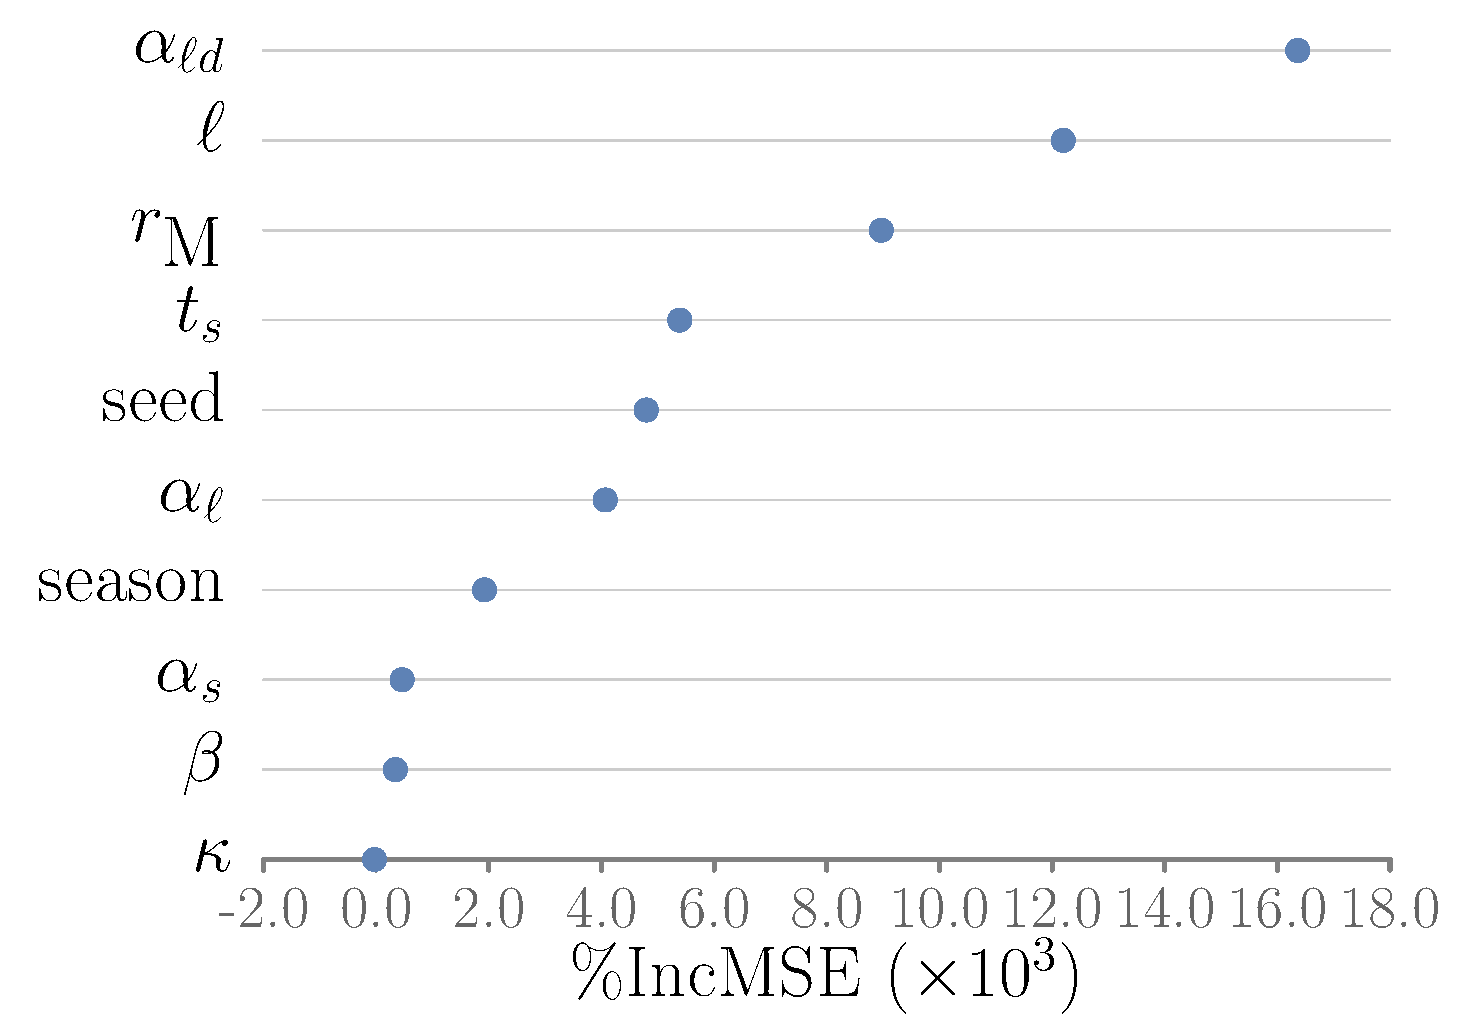
\includegraphics[width=1.1\textwidth]{../clustering/results/rf_importance_cluster_mse_all.pdf}
%%     \caption{All \label{fig:rfAll}}
%% \end{subfigure}
%% %%
%% \begin{subfigure}[b]{.32\textwidth}
%%     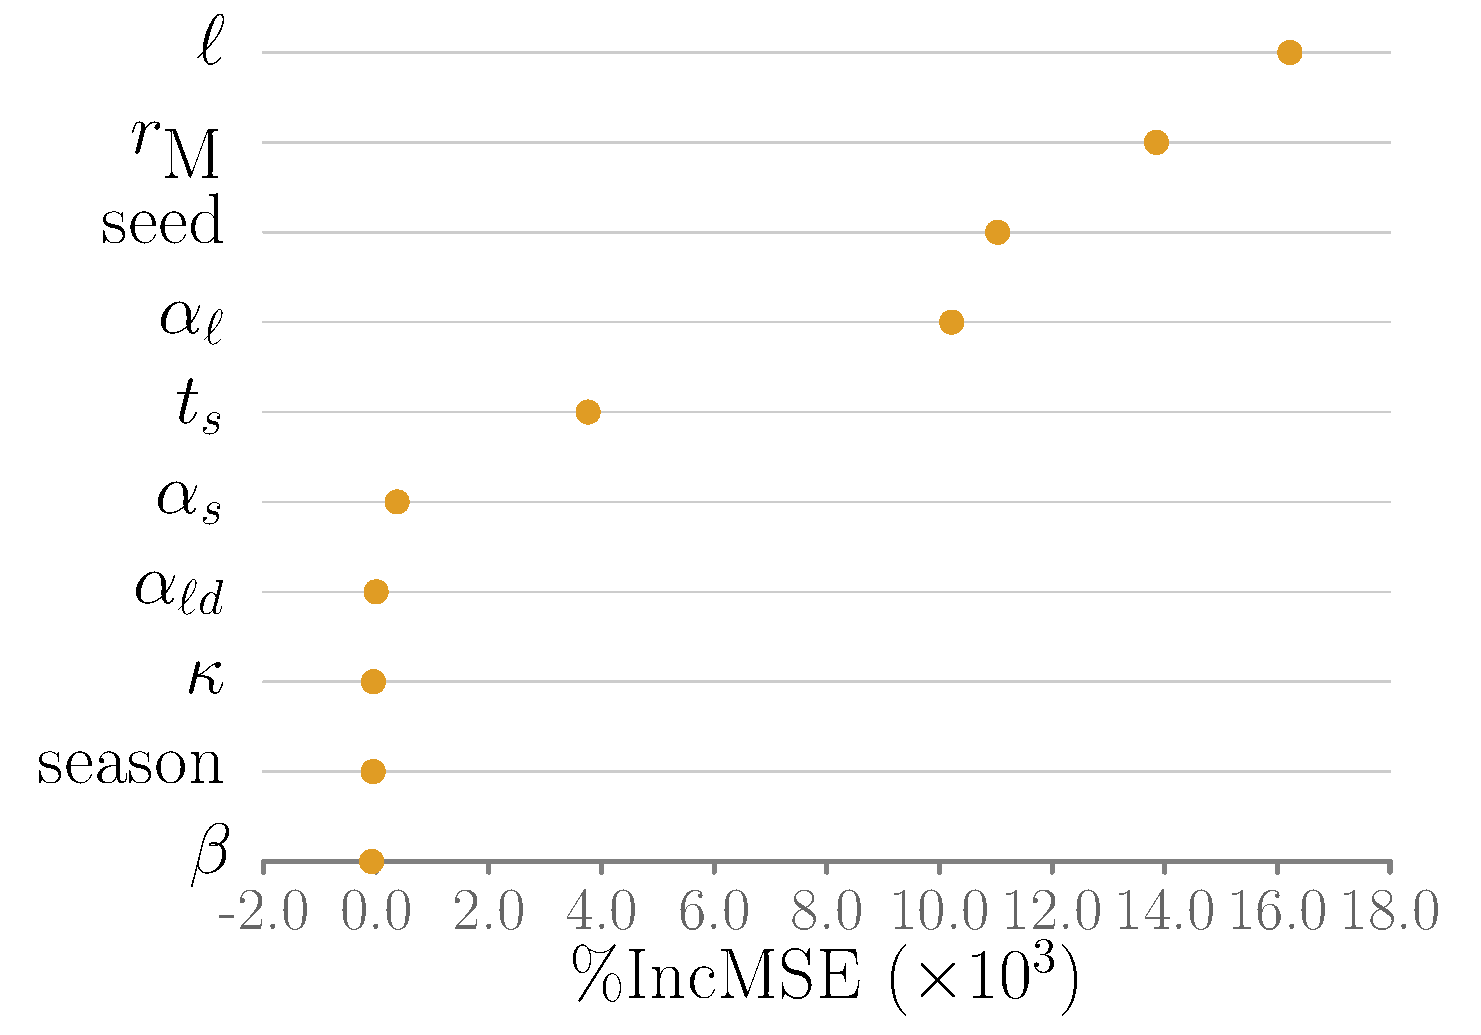
\includegraphics[width=1.1\textwidth]{../clustering/results/rf_importance_cluster_mse_A.pdf}
%%     \caption{Class A\label{fig:rfA}}
%% \end{subfigure}
%% %%
%% \begin{subfigure}[b]{.32\textwidth}
%%     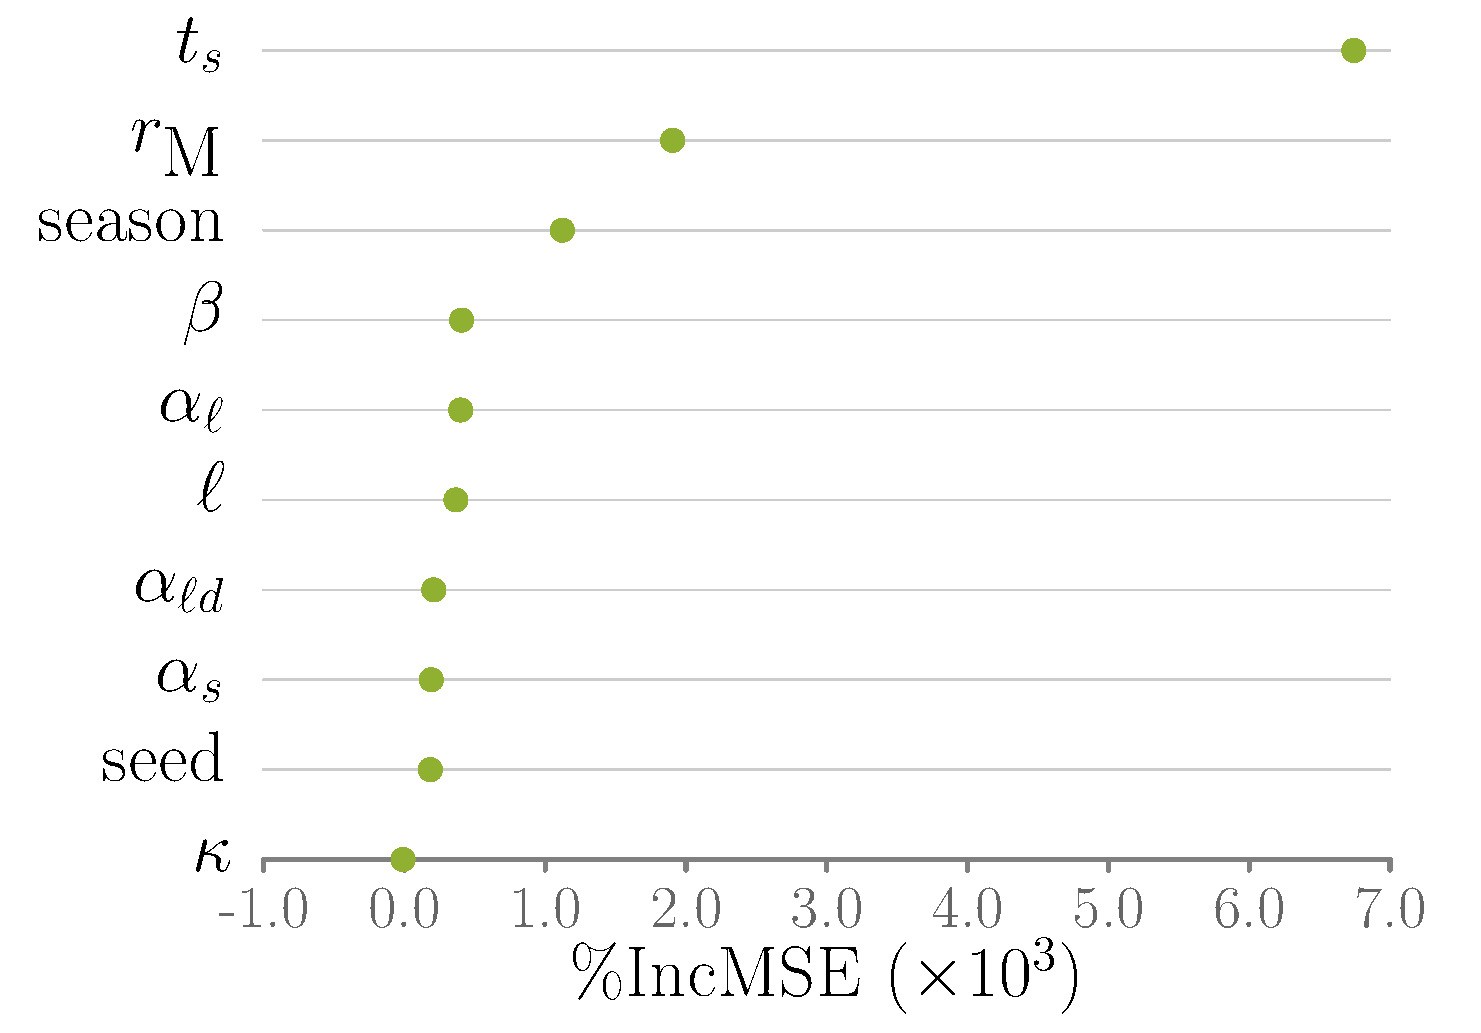
\includegraphics[width=1.1\textwidth]{../clustering/results/rf_importance_cluster_mse_B.pdf}
%%     \caption{Class B\label{fig:rfB}}
%% \end{subfigure}
%% %%
%% \begin{subfigure}[b]{.32\textwidth}
%%     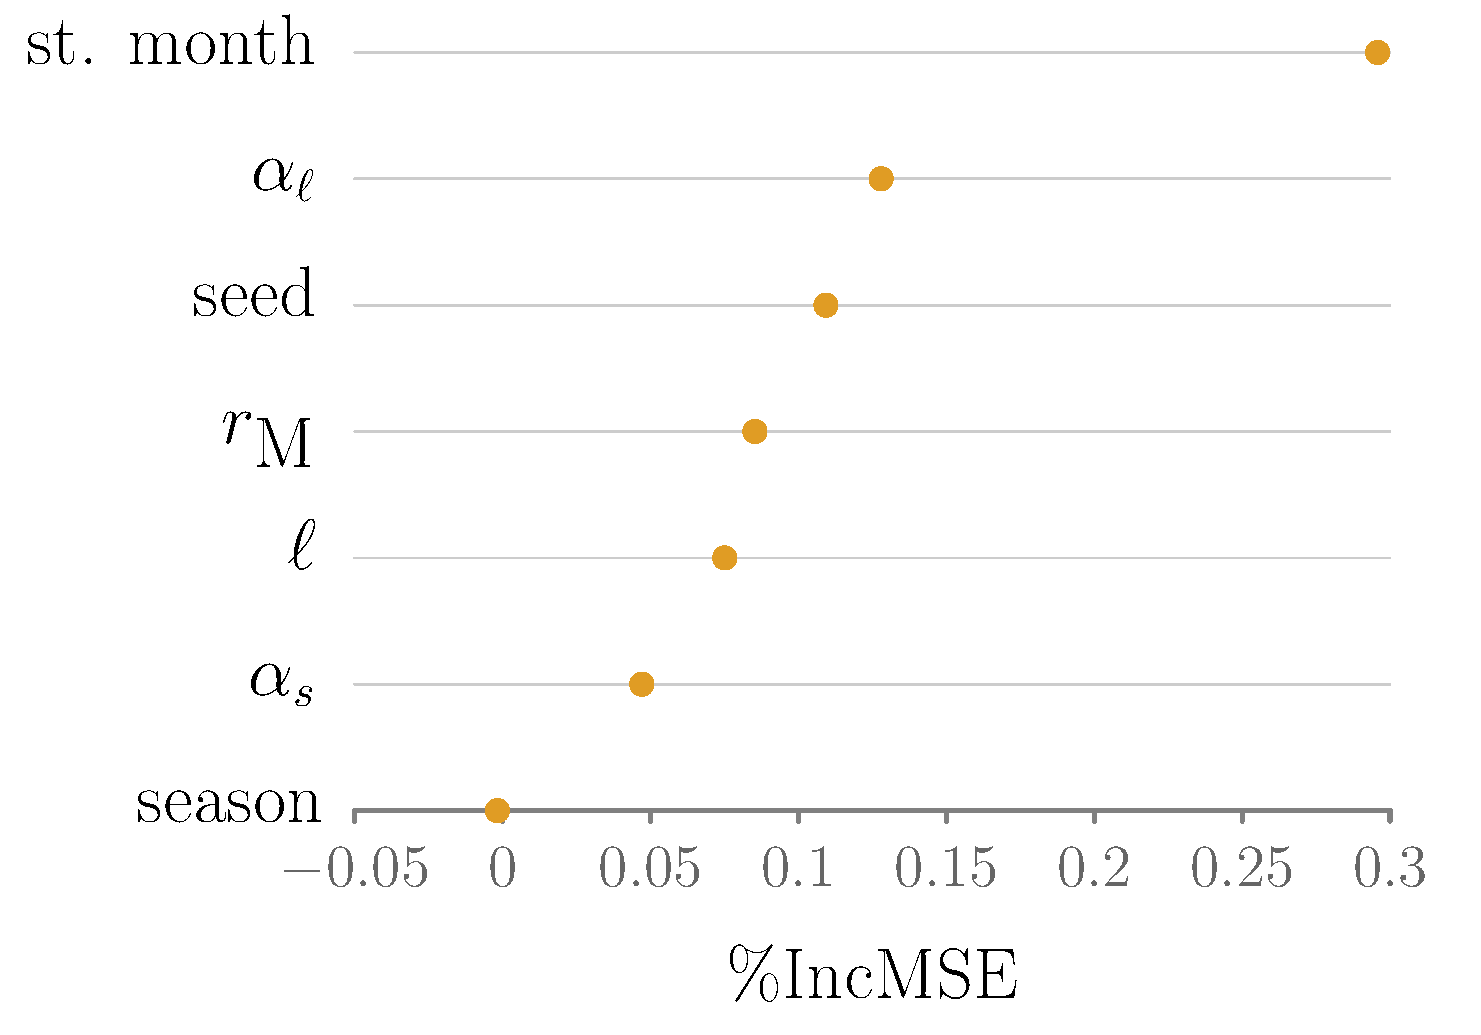
\includegraphics[width=1.1\textwidth]{../cellular_automata/results/rf/rf_importance_short_mse.pdf}
%% \caption{Class A\label{fig:rfShort}}
%% \end{subfigure}
%% %%
%% \begin{subfigure}[b]{.32\textwidth}
%% 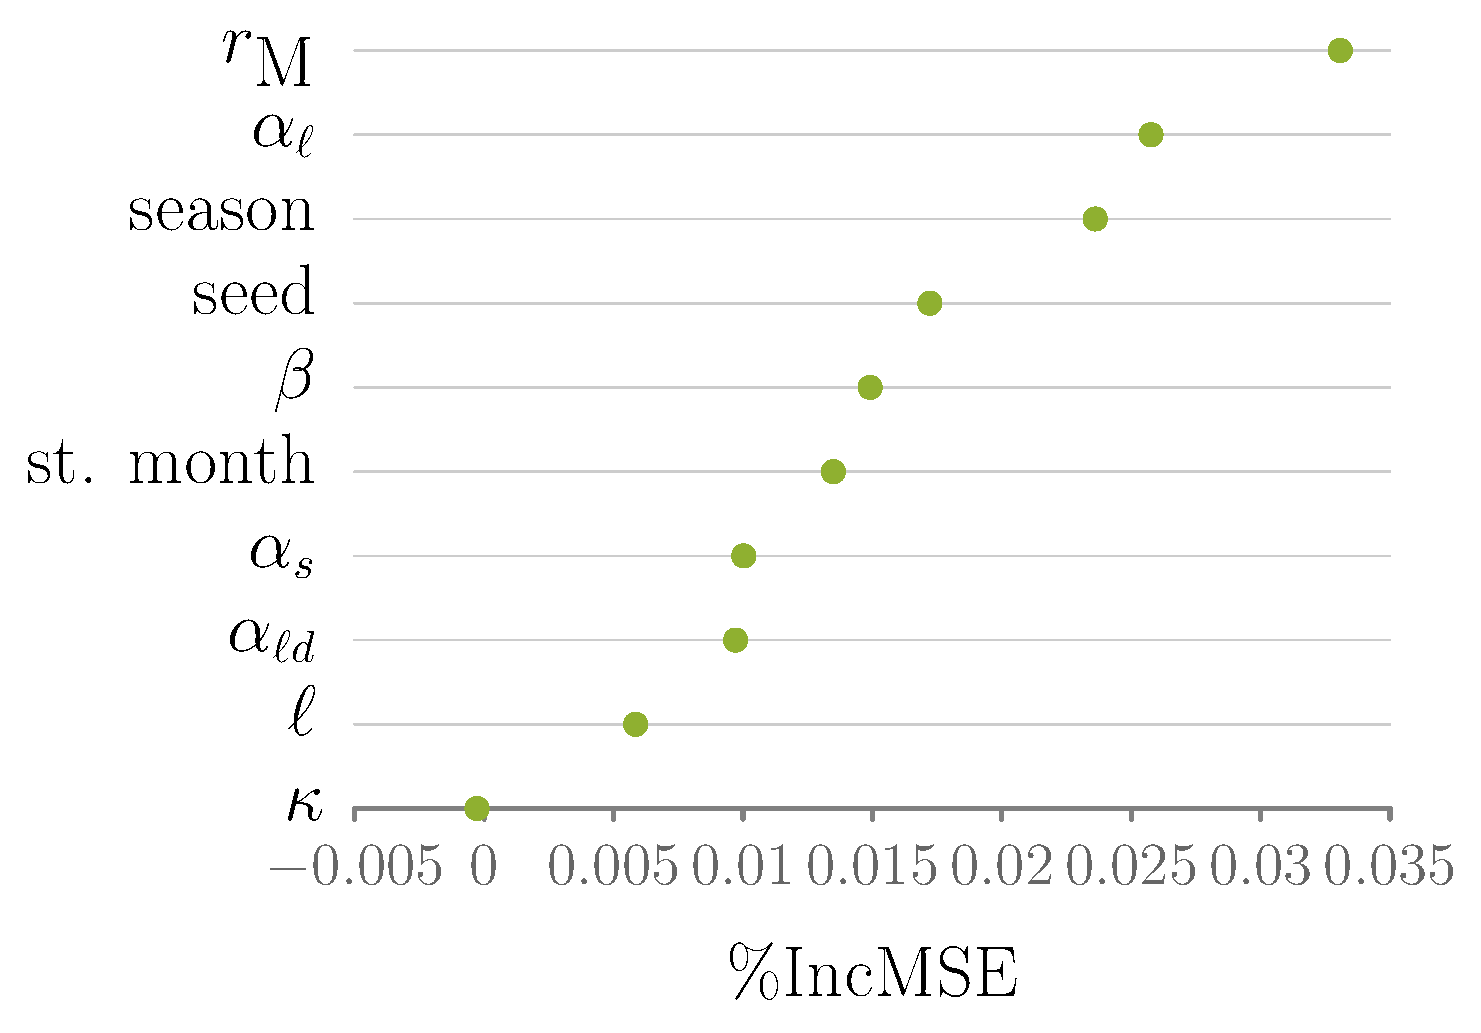
\includegraphics[width=1.1\textwidth]{../cellular_automata/results/rf/rf_importance_long_mse.pdf}
%% \caption{Class B\label{fig:rfLong}}
%% \end{subfigure}
%%\caption{\textbf{Parameter importance.} Random
%%Forest~\cite{breiman2001random} method was applied to study parameter
%%importance. (a)~With cluster index as the dependent variable,
%%the analysis was performed on the set of model instances which yielded a
%%similarity~$\similarity\ge6$.
%%%% (b)~The sensitivity of the spread pattern to parameters was analyzed by
%%%% repeating the same process, but with cluster index as the dependent
%%%% variable.
%%The results for the entire set (a) and separately for Class~A (b) and
%%Class~B models (c) are shown. The parameters are ordered by their
%%importance based on percentage increase in mean square error from permuting
%%the variable--higher, the more important.
%%\label{fig:sensitivity}}
%%%% a total of $17,000$ samples from the parameter space
%%\end{figure}
%%
%% Class~B models show more sensitivity to start time step of simulation than
%% Class~B models. The main reason why it is not at all critical in the latter
%% class is because the pest was reported just before the rainy season;
%% subsequent months have lean trade flows, and as a result it does not affect
%% the spread much. However, it does not seem to have much effect on the
%% radial spread component as is the case with Class~A models. In both cases,
%% the spread is very sensitive to the local human-mediated pathway
%% parameter~$\afm$. In the case of Class~A models, this pathway leads to
%% faster spread within localities. In Class~B models, higher the value, the
%% greater the chance of long-distance spread as it quickly leads to infection
%% of large portions of the localities, and therefore their total
%% infectiousness. Later, we will discuss on how it influences the spread rate
%% for the rest of the region.
%% \begin{figure}[ht]
%%     \centering
%%     \begin{subfigure}[b]{.48\textwidth}
%% 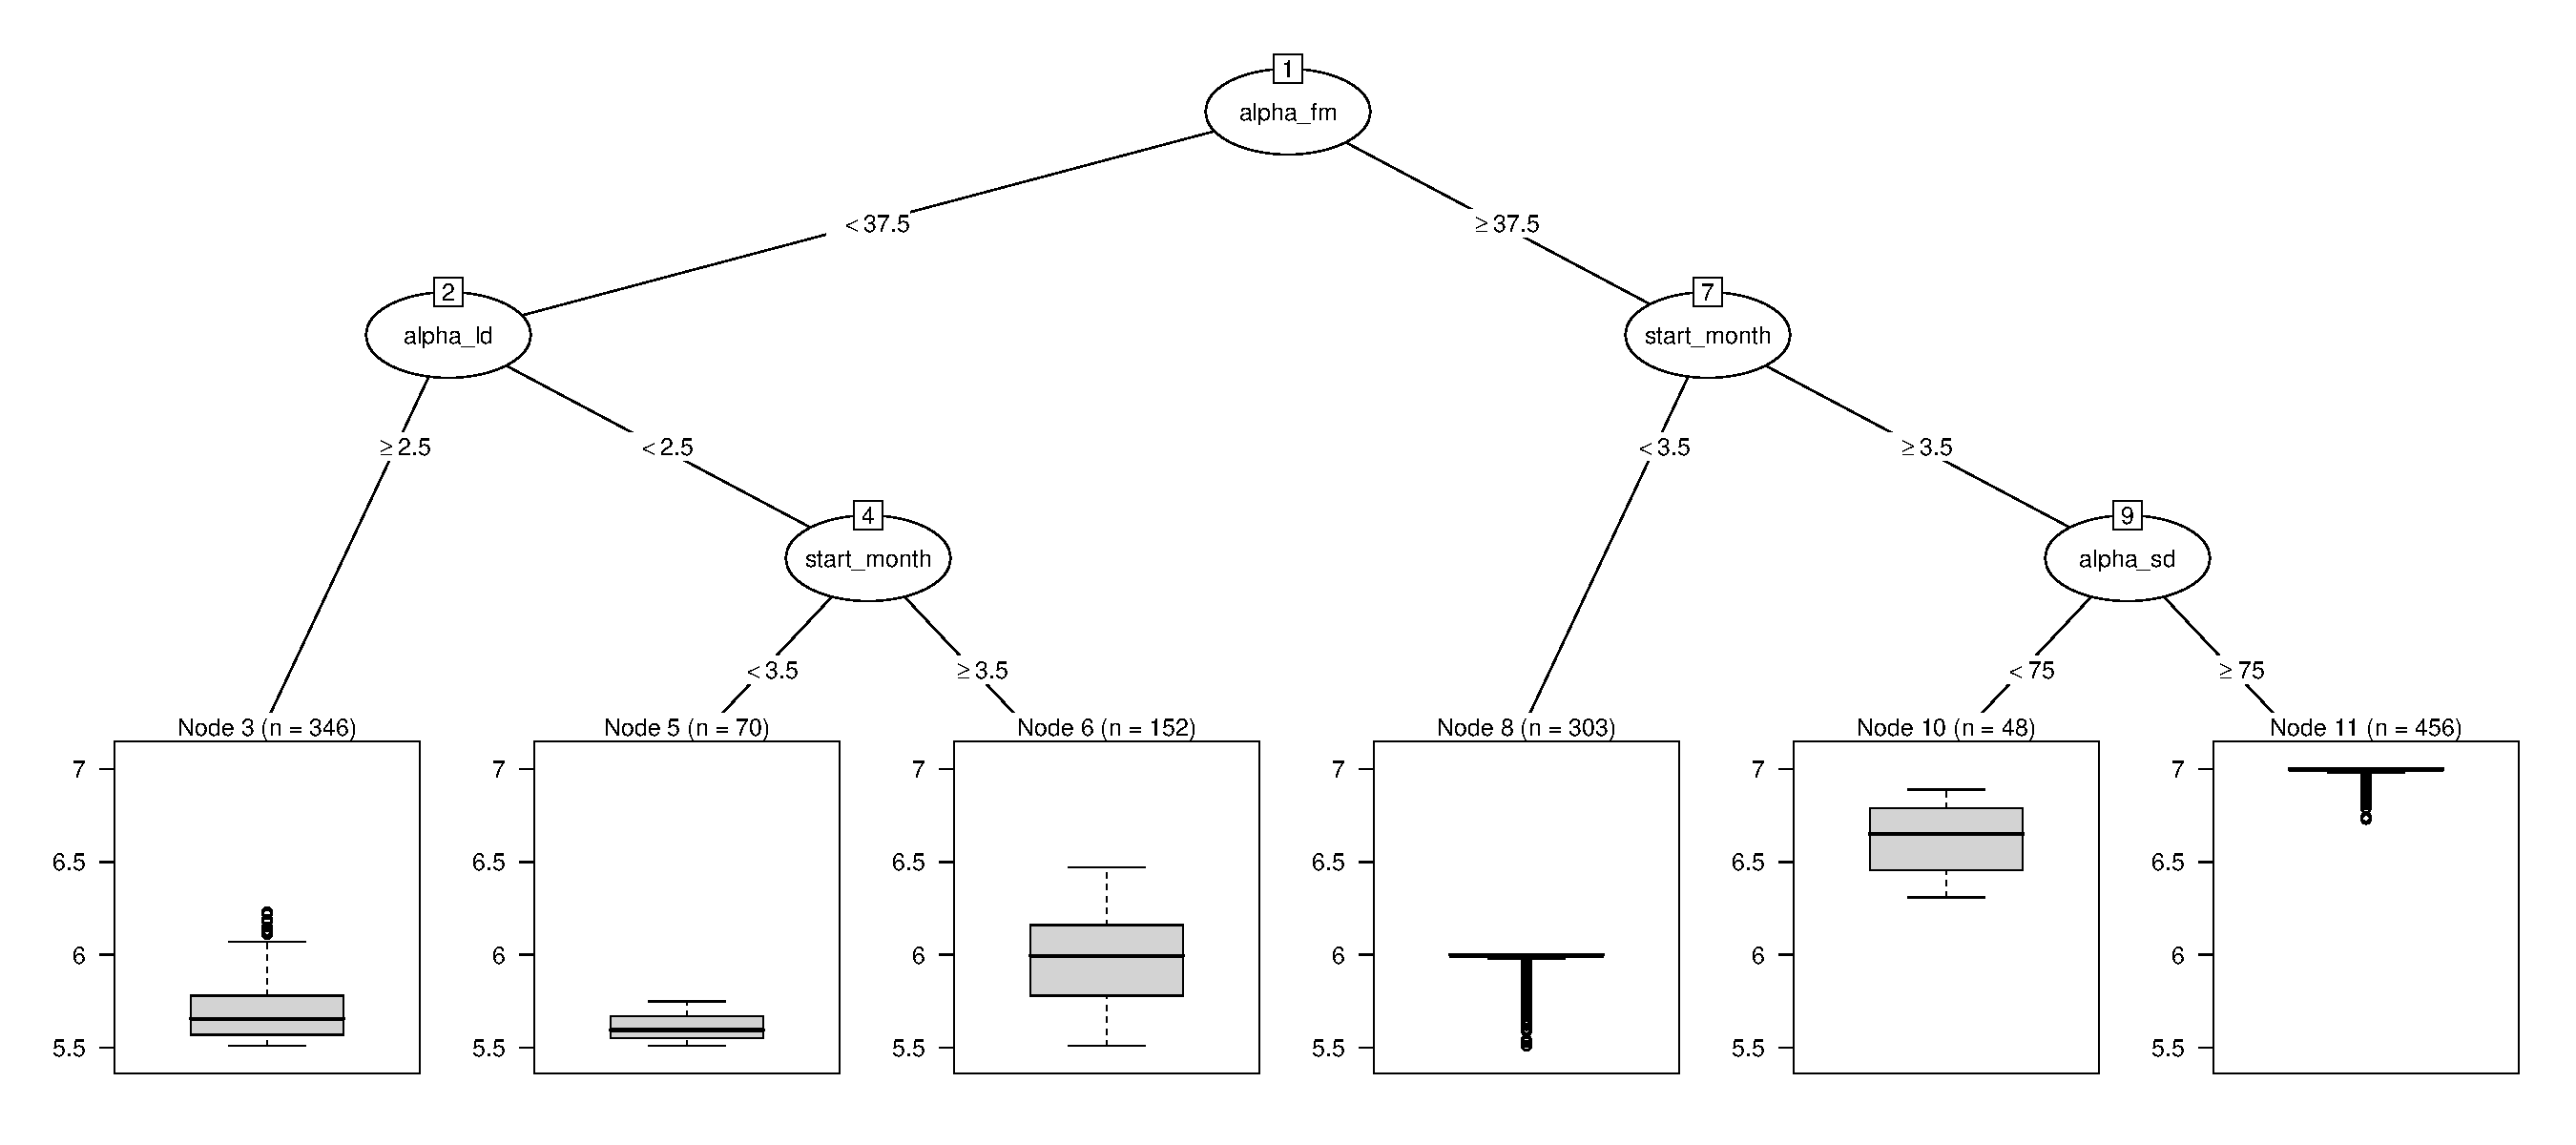
\includegraphics[width=\textwidth,trim={1cm 1cm 1cm 1cm},clip]{../cellular_automata/results/cart/m2_l2_tree.pdf}
%%     \caption{$\mooreRange=2$, $\ell=2$ \label{fig:cart22}}
%%     \end{subfigure}
%%     \begin{subfigure}[b]{.48\textwidth}
%% 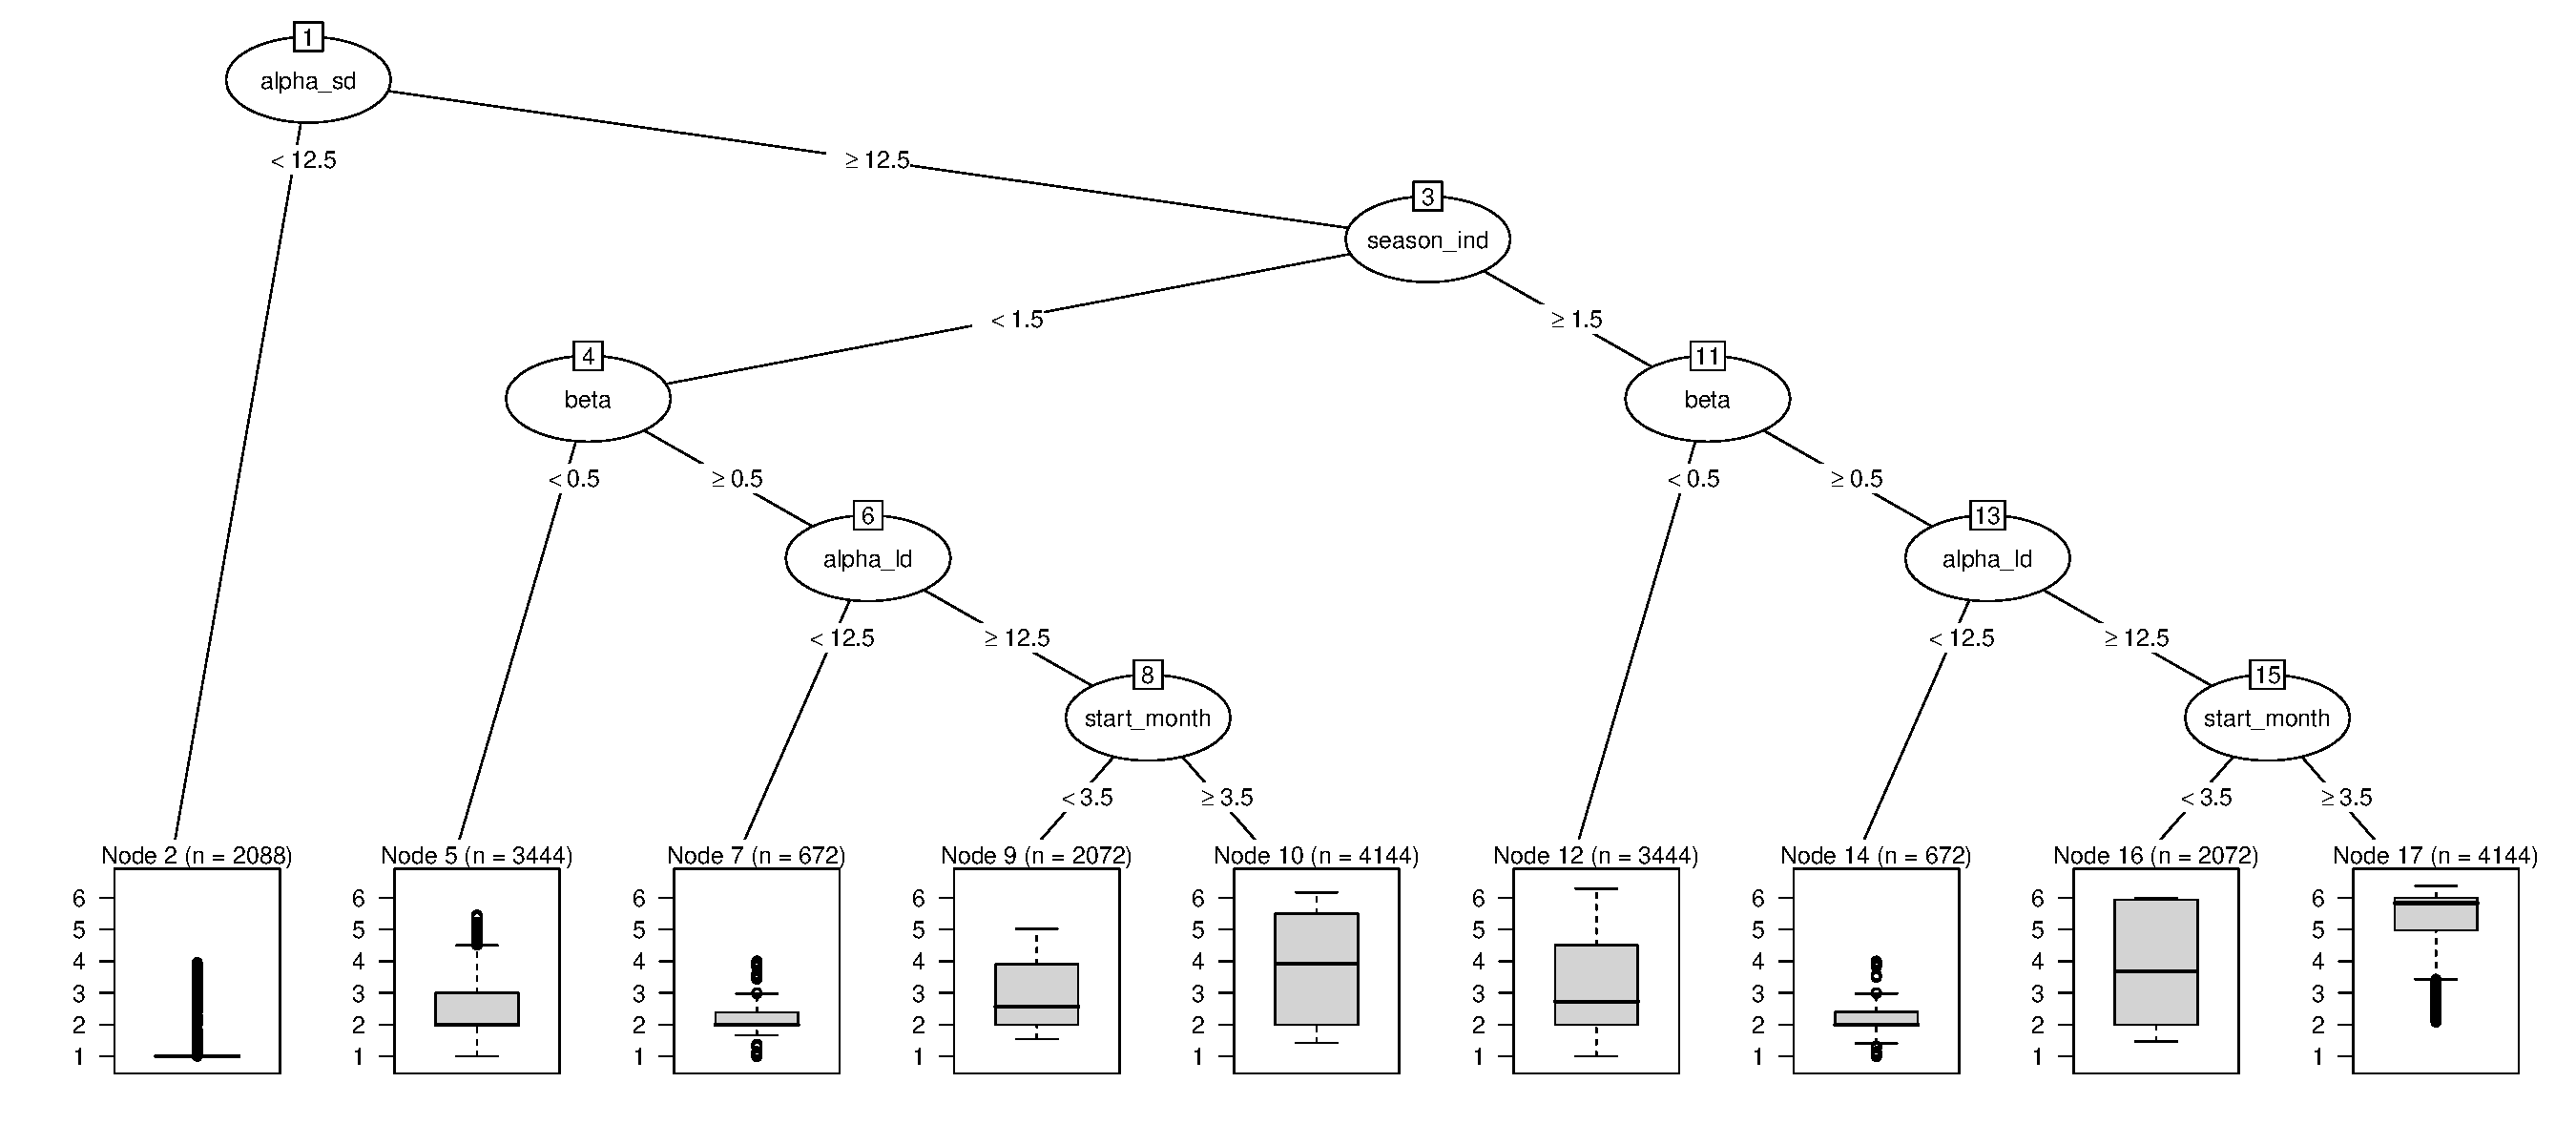
\includegraphics[width=\textwidth,trim={1cm 1cm 1cm 0cm},clip]{../cellular_automata/results/cart/m2_l3_tree.pdf}
%%     \caption{$\mooreRange=2$, $\ell=3$ \label{fig:cart32}}
%%     \end{subfigure}
%%     %% \begin{subfigure}[b]{.48\textwidth}
%%     %% 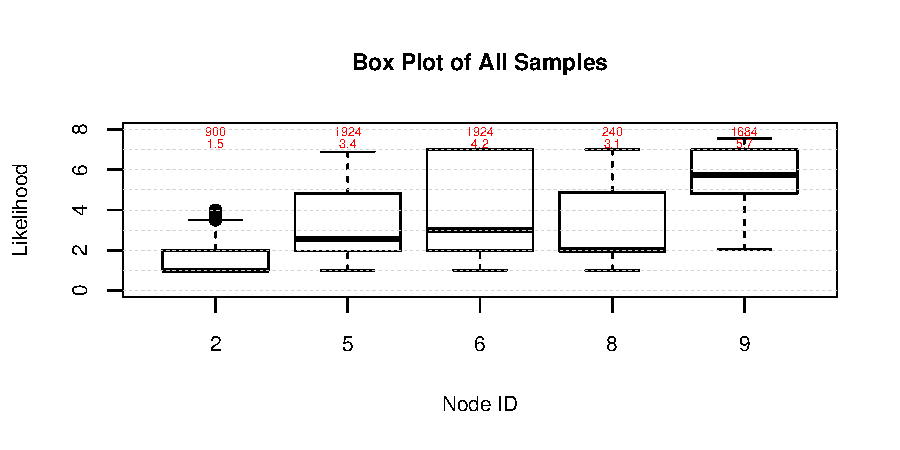
\includegraphics[width=\textwidth]{figs/cart_box1.pdf}
%%     %% \caption{\label{fig:cartBox1}}
%%     %% \end{subfigure}
%%     %% \begin{subfigure}[b]{.48\textwidth}
%%     %% 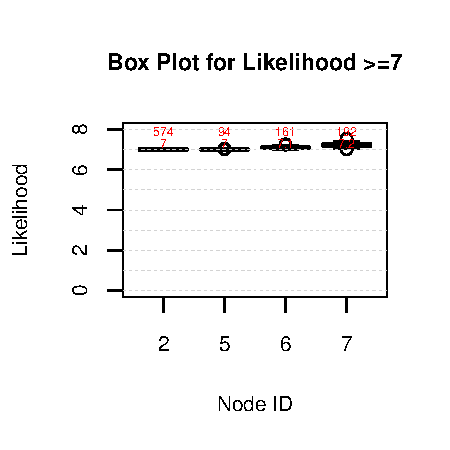
\includegraphics[width=\textwidth]{figs/cart_box2.pdf}
%%     %% \caption{\label{fig:cartBox2}}
%%     %% \end{subfigure}
%%     \caption{CART analysis of the parameter space: The models with
%%         similarity$\ge5.5$ were partitioned based on the Moore
%%     range~$\mooreRange$ and latency period~$\ell$ tuple and analyzed. Two
%%     of the nine cases are shown. The complete set is in
%%     Figure~\ref{S:fig:cart}.}
%% \end{figure}
%%

%% The rest of the section will focus more on Class~B
%% 
%% See
%% Figures~\ref{S:fig:cartAgglomerative}(b)
%% and~\ref{S:fig:cartkmeans}(a) in the supplement. We have also considered
%% the case of more than two clusters. This is analyzed in the following
%% section. Our
%% results remain consistent across the different clustering methods applied.
%% 
%% %% It is characterized by %%
%% a combination of Moore range ($\mooreRange$), latency period ($\ell$) and
%% %% pathway parameters~$\asd$ and~$\afm$ that lead to rapid spread between
%% %% adjacent cells.  
%% As described in Methods, the goodness of fit of a model configuration was
%% evaluated by comparing the corresponding simulation output with ground
%% truth from Bangladesh using the similarity score in~\eqref{eqn:similarity}.
%% Variability in the spread patterns was studied by clustering the simulation
%% outputs of the selected configurations (Figure~\ref{fig:clusterOutline})
%% and analyzing the relationship between the resulting clusters and model
%% parameters. 
%% 
%% Even though
%% each of these models are a close match to the ground truth, two spread
%% patterns can be very different from each other. 

%% The results from this study was that with seeding in Spain, Tuta would
%% spread radially. This is due to taking into account only short distance
%% spread, and the fact that no area was unsuitable year-round. They
%% introduced parameters in stages, first considering only NDVI, and assuming
%% that temperature and humidity reached the thresholds. In this scenario,
%% Tuta spread to every region of Africa, excluding Madagascar, in 6 years.
%% When including temperature as a parameter as well, Tuta spreads to all of
%% Africa, excluding Madagascar, in 9 years. When taking into account NDVI,
%% temperature, and humidity as described above, every region of Africa is
%% invaded in 9 years (excluding Madagascar), except for regions in the Sahara
%% desert, which is in the exposed state.


%\aacomment{This part will be moved to results}
%\aacomment{Need to describe each scenario: how the initial seeds were
%decided, the basis for choosing them. I think it is a good idea to also
%name them (Scenario A, B, C, etc.)}


%% We used the CA model by Guimapi~et.~al.~\cite{guimapi2016modeling} as a
%% baseline for our study. We will test three scenarios using this model in Southeast Asia. Scenario A seeds the region of Chin in northeast Myanmar. This region represents a possible pathway of \tuta{} should it spread radially through the border with Bangladesh. Scenario B seeds the region of Johor in Malaysia - including Singapore. This region contains major ports in Malaysia including Tanjung Pelepas \cite{khalid2005}, and Singapore is also a major trading hub for Bangladesh. Scenario C seeds the region of Putrajaya, which is the region which includes the largest port in Malaysia \cite{khalid2005}. Scenario D seeds the region of Penang, which is also a major port \cite{khalid2005}. Scenario E seeds Sarawak which is one of the Malaysia districts not in the mainland. This district contains another major port: Bintulu \cite{khalid2005}. Each scenario is simulated with Moore neighborhoods of 2 and 3, and follow the rules as in \cite{guimapi2016modeling}. Our grid resolution is 0.25x0.25 degrees. This corresponds to about 27.75 km at the equator. Thus one cell will be roughly 25x25 km as in above. We consider Moore neighborhoods of 2 and 3 to reflect 50 - 75 km range. For NDVI data, our resolution is small, so we choose the maximum NDVI for a grid cell.\\



It is possible that there
is lot of variation in consumption within a country as well as across
seasons. The relationship between trade volume and distance between
localities could vary from one region to another. Extending to other
regions such as North America, China or Australia, might require accounting
for seedling trade and greenhouse production.
One way to increase our understanding
is to analyze regions in Europe and Africa where \tuta{} has been present
for more than a decade to better calibrate our models. However, one needs
to be cautious while applying studies of one region to another. For
example, in Europe and parts of Africa seedling trade and greenhouse
cultivation play an important part in tomato production~\cite{}. 
%% Nopsa~et~al.~\cite{nopsa2015ecological} considered this problem in the
%% context of soybean rust in the US, modeling the spread as a propagation
%% process over a network of counties. They developed efficient strategies to
%% reduce the spread by identifying and monitoring only a subset of locations
%% which are critical for the spread.
%% Nevertheless, we considered the scenario in which \tuta{}
%% establishes in the region between Kuala Lumpur and Singapore. The
%% simulations suggest that the pest will spread to most localities in
%% Malaysia and Sumatra, Indonesia within an year.
%% 
%% Our
%% results show that for all countries, once the pest is introduced, within
%% 2-3 years the it will spread to almost all localities, and when it reaches
%% a high production locality, it spreads to other regions within a year.
%% Past invasion records support this trend.
%% The pest became widespread in
%% countries Mediterranean
%% region, in Middleeastern countries, and in India in just 2-3 years.

%%   

%% We
%% considered two hypothetical scenarios: (i)~\tuta{} is introduced to the
%% Palawan region from Malaysian Borneo (natural pathway) and (ii)~it is introduced to the high
%% production area of Northern Mindanao. While in the first case we did not
%% observe spread beyond the Palawan region, in the second case, within two
%% years, almost all localities were invaded. The latter case is shown in
%% Figure~\ref{fig:phlBContour}.
%% However, we recall that trade between some countries was ignored, and as a
%% result our model might have missed some long-distance jumps.  For example,
%% from Vietnam, there is a possibility that it can enter Phnom Penh, Cambodia
%% through tomato imports during the rainy months~\cite{sokhen2004}. The
%% southwards spread to Malaysia might be faster than predicted by Class~B
%% spread due to exports from Thailand to Malaysia and Singapore.
%%
%% Class~A predicts that the entire Mainland Southeast Asia will be infested
%% with four years.
%% %% We considered three scenarios of introduction of the pest to the region.
%% %% The first scenario corresponds to evolution of the spread from Bangladesh
%% %% (B1). The other two are hypothetical scenarios based on the analysis in
%% %% Section~\ref{sec:entry}. Scenario~M corresponds to \tuta{} introduced near
%% %% a major port region of Malaysia. The third Scenario~P is its introduction
%% %% to Philippines close to the captial city Manila assuming introduction
%% %% due to migratory workers from \tuta{} affected regions.
%% 
%% From Figure~\ref{fig:totalSpread}, we observe that the range expansion is
%% much faster with Class~A compared to Class~B. The main reason for the slow
%% spread is due to not accounting for trade interactions between countries in
%% the model. The spread is characterized by slow spread between countries and
%% rapid expansion within. For example, the big jumps in range expansion
%% between time steps 72 and 120 is mainly due to spread within Myanmar
%% through long-distance jumps. The challenges in modeling international trade
%% are covered in Methods (Trade flows). But when we consider the global
%% spread pattern of \tuta{}, we observe reduction in rate of range expansion
%% in certain regions.
%% 
%% Also, the predicted spread could be
%% slower due boundary effects; we have not accounted for cells belonging to
%% Northeastern parts of India that share border with Bangladesh and Myanmar
%% and the Yunnan province of China.  On the other hand, when we focus on each
%% country separately (Figure~\ref{fig:spreadWithin}, we observe that the
%% spread within a country is much faster in the case of Class~B.  Results
%% suggest that major production areas of a country will be invaded within 2-3
%% years of introduction.
%% 
%% The spatio-temporal spread for Scenario~B1 is shown in
%% Figure~\ref{fig:spreadBGD}. The start time corresponds to~24 time steps (or
%% two years) from the first report. The results indicate that there is a high
%% chance that \tuta{} will spread to Mainland Southeast Asia in four to six
%% years. Because of long distance dispersal, we also observe a non-radial
%% spread. Aided by domestic trade and exports from Thailand, there is
%% possibility that the pest will be introduced to Peninsular Malaysia and
%% subsequently to Singapore and Indonesia in this period even though this
%% area is much farther from the current range of \tuta{}. Also, we see the
%% possibility of the pest crossing the sea from Peninsular Malaysia to
%% Malaysian Borneo within a year of introduction to this country. However,
%% these are conservative estimates. First of all, the simulations do not
%% account for possible new introductions. 

%% The spread due to other two scenarios are shown in Figures~\ref{spreadMYS}
%% and~\ref{spreadPHL} respectively. Note that in both of these scenarios we do not
%% account for the spread from Bangladesh. This is crucially dependent on the
%% time of introduction. However, it is critical to consider the synergistic
%% effects of range expansion from multiple locations. The spread in
%% Scenario~M follows a similar pattern as in Scenario~B3.
%% \aacomment{Philippines pending}.

%% \begin{figure}[ht]
%%     \centering
%%     \begin{subfigure}[b]{.32\textwidth}
%%         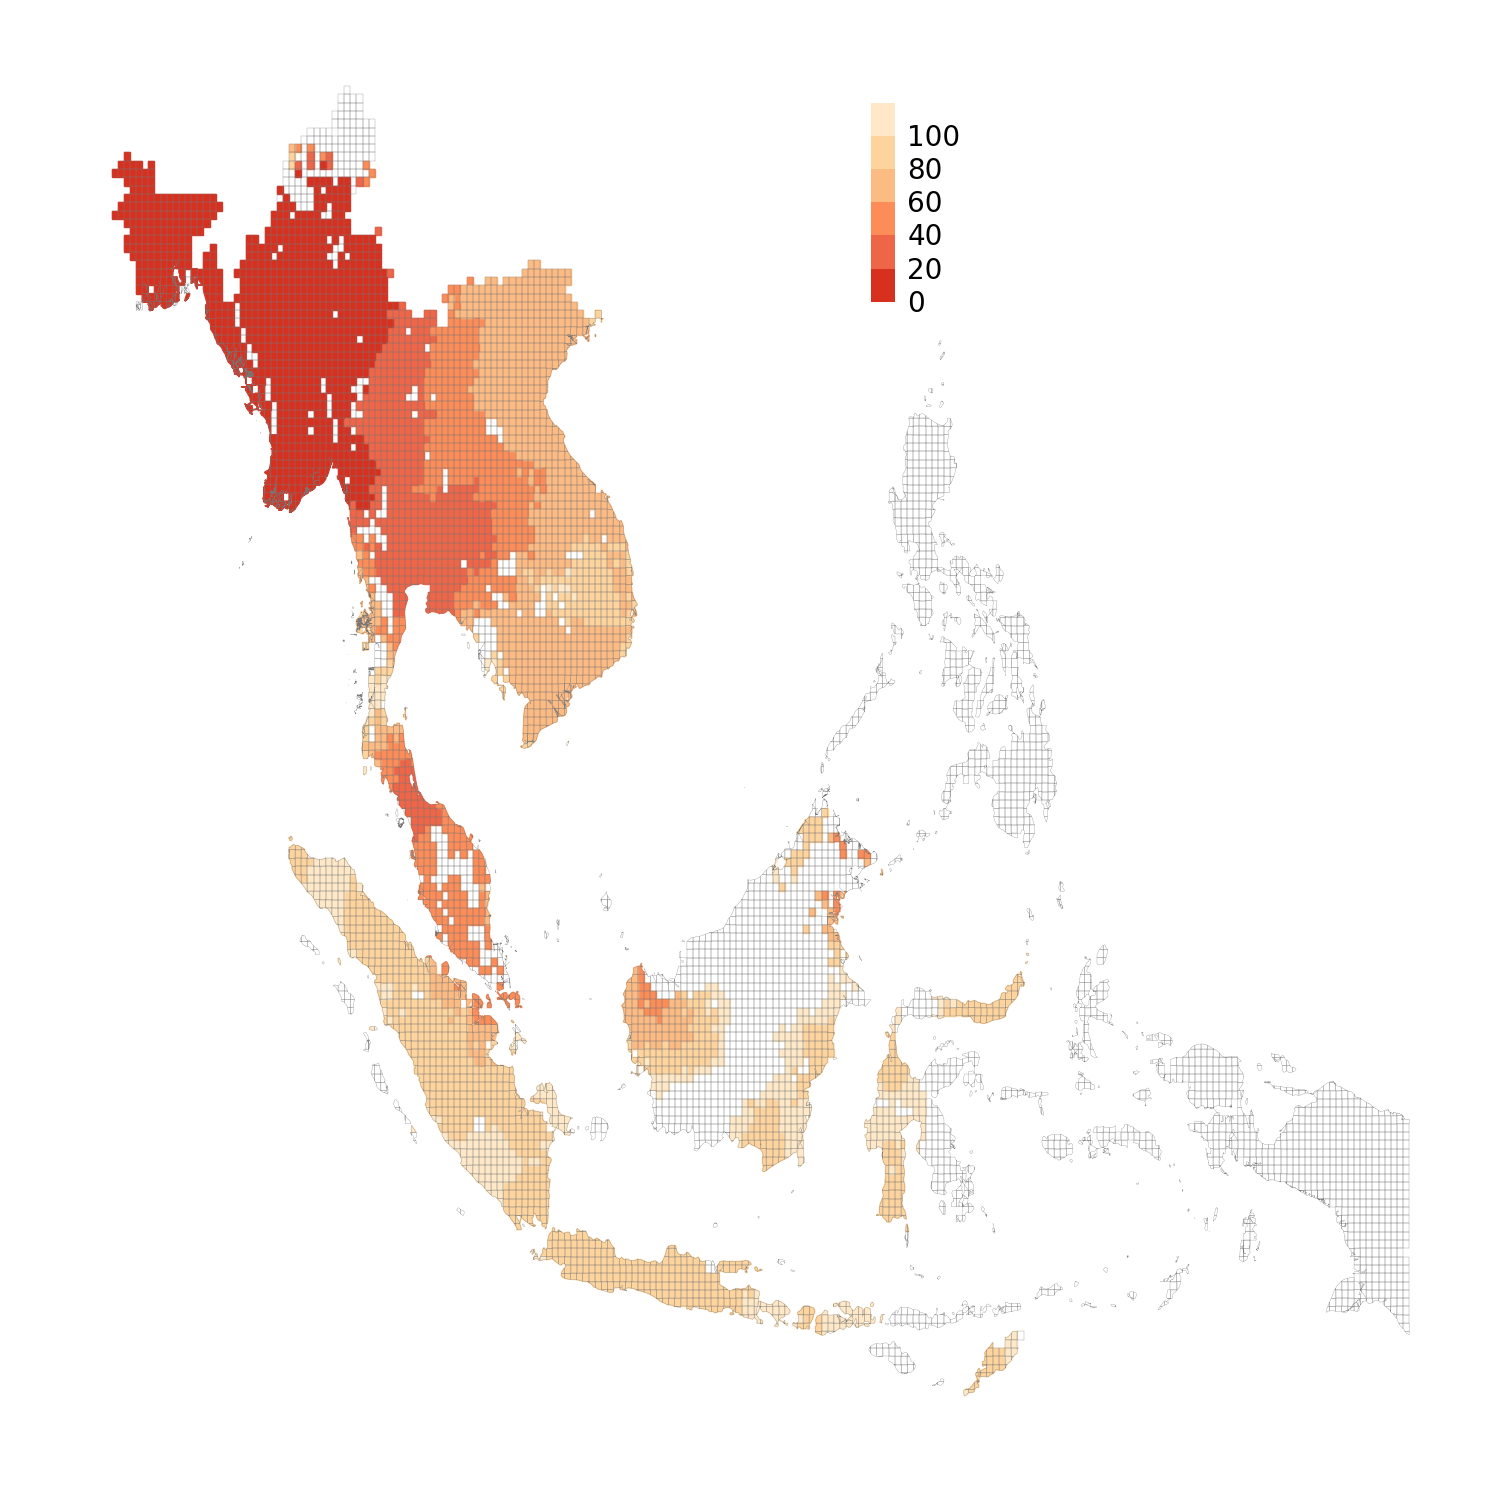
\includegraphics[width=\textwidth,trim={3cm 3cm 8cm 3cm},clip]{figs/spread_BGD.png}
%%     \caption{Scenario~B1\label{fig:spreadBGD}}
%%     \end{subfigure}
%%     \begin{subfigure}[b]{.32\textwidth}
%%         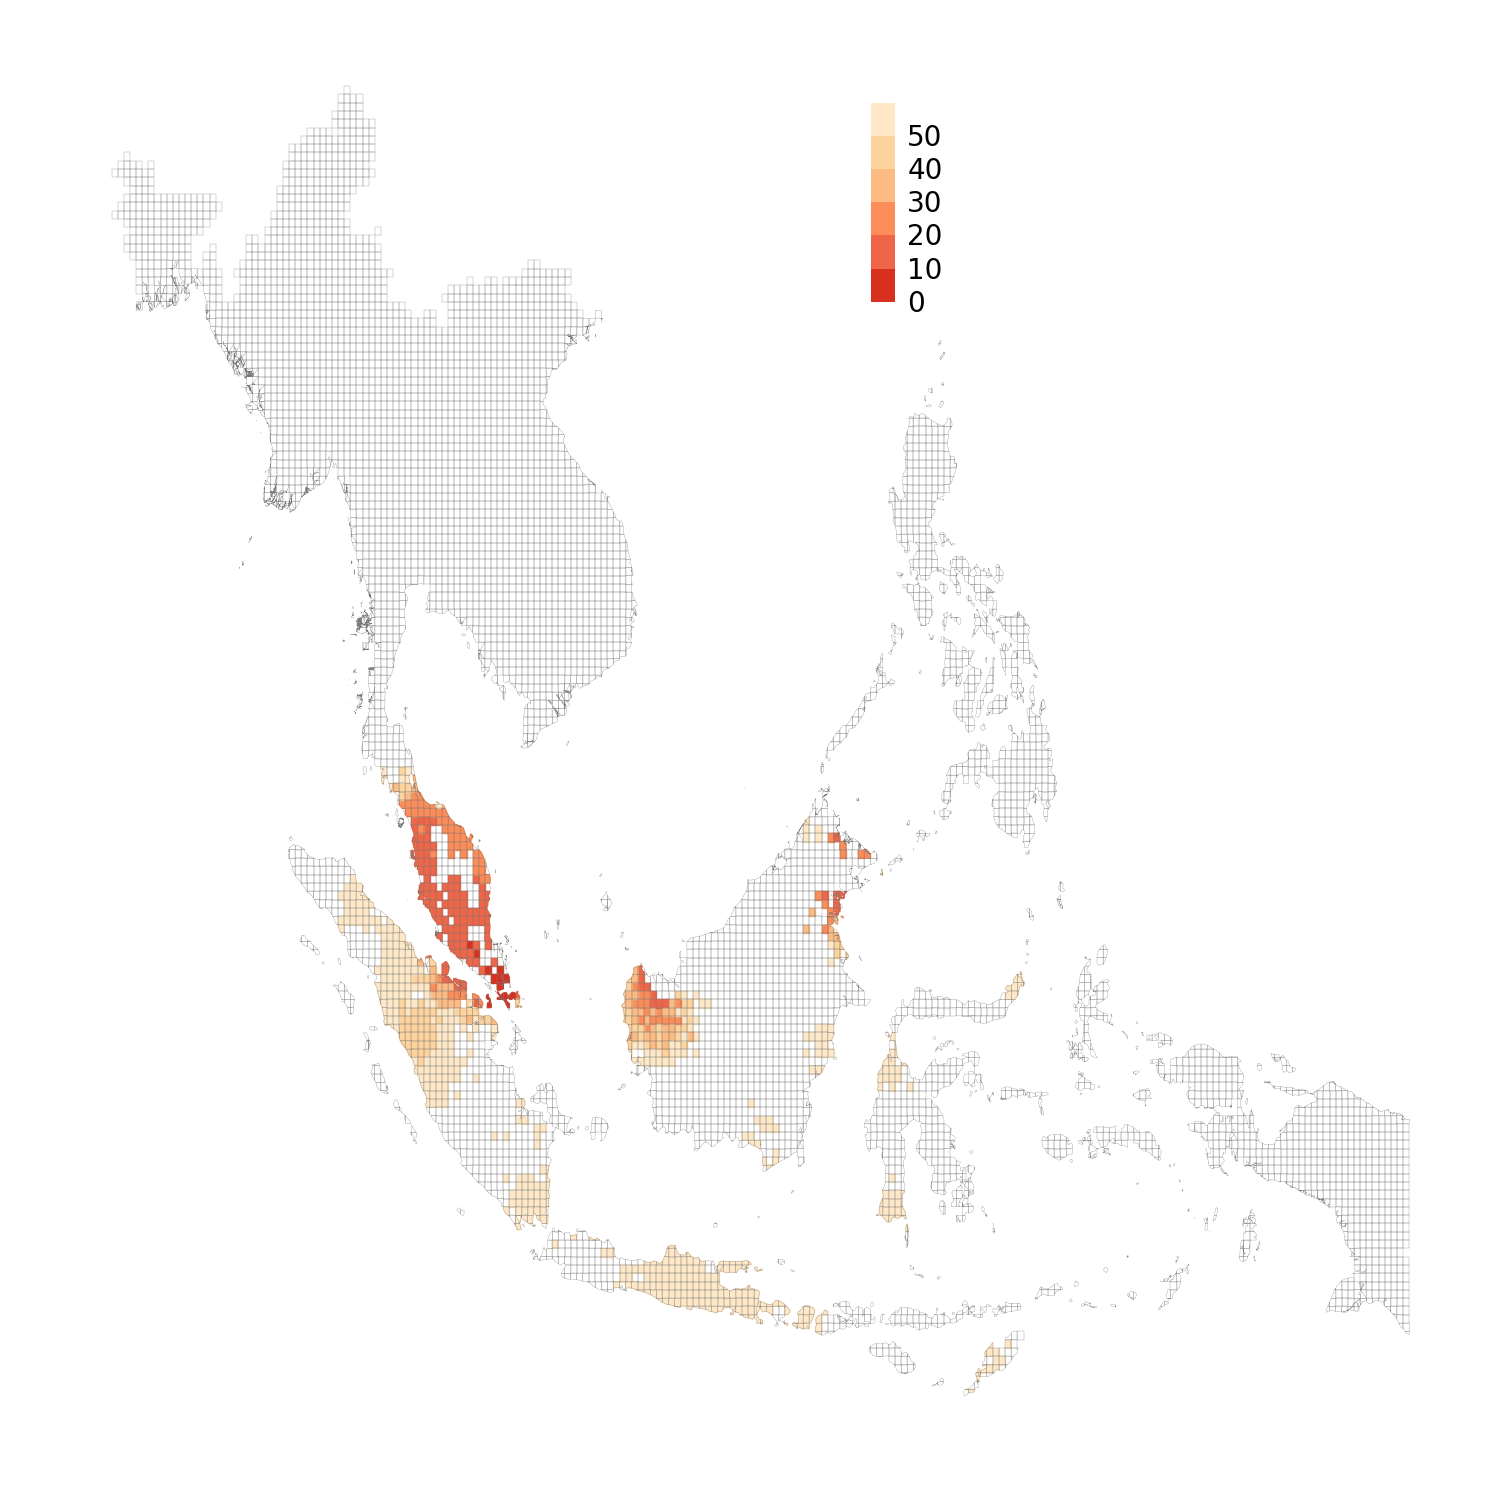
\includegraphics[width=\textwidth,trim={4cm 2cm 8cm 12cm},clip]{figs/spread_MYS.png}
%%     \caption{Scenario~M\label{fig:spreadMYS}}
%%     \end{subfigure}
%%     \begin{subfigure}[b]{.32\textwidth}
%%         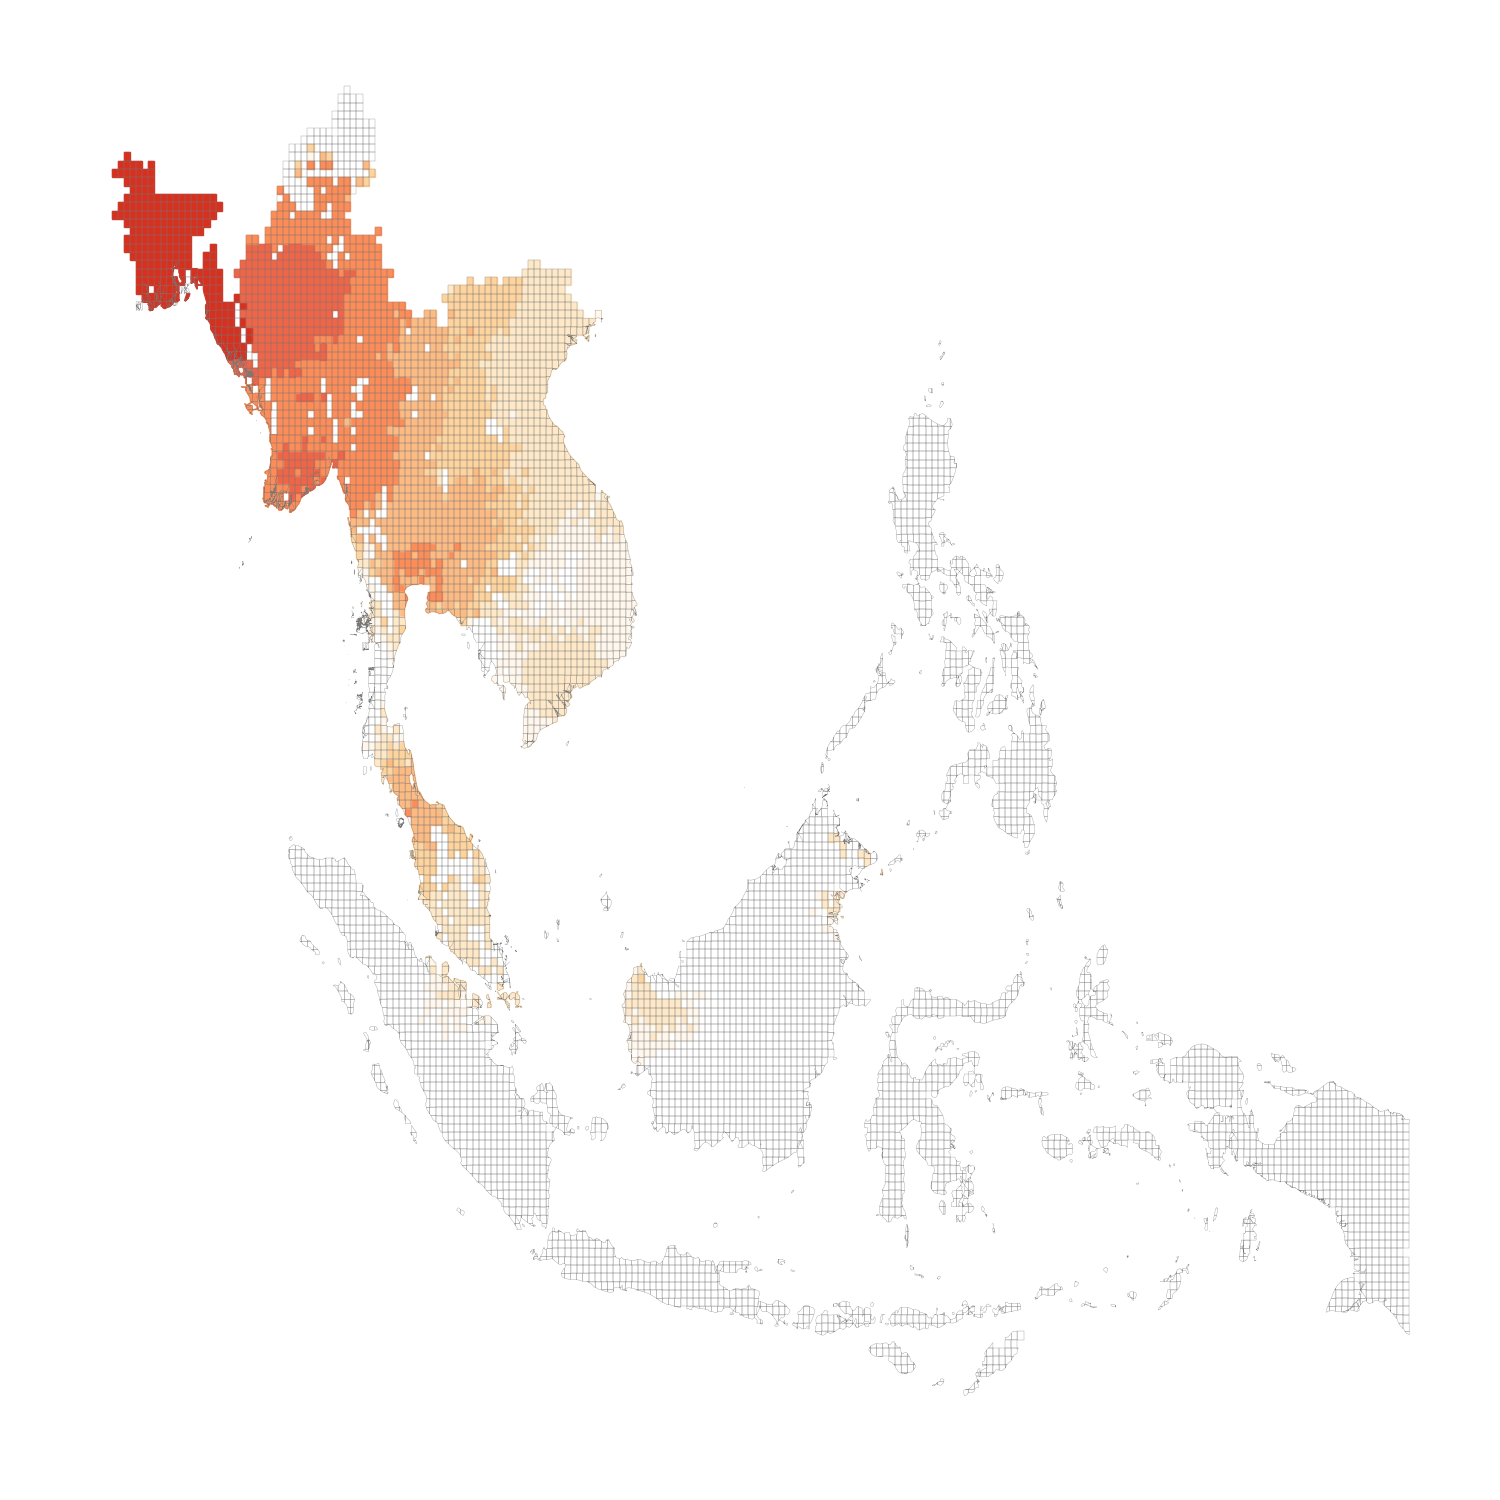
\includegraphics[width=\textwidth,trim={4cm 2cm 8cm 12cm},clip]{figs/spread_PHL.png}
%%     \caption{Scenario~P\label{fig:spreadPHL}}
%%     \end{subfigure}
%%     \caption{Possible spread of \tuta{} in the focus region under three
%%     scenarios. In each plot, the legends correspond to months. For the
%%     purpose of plotting, for each cell, we compute the time~$t$ for which
%%     the empirical probability of infection before~$t$ is at least $0.1$.
%%     Scenario~B3 starts with Bangladesh and significant parts of Myanmar
%%     infested accounting for spread from May 2016 to May 2018.
%%     \aacomment{Philippines pending, legend will be made bigger}}
%% \end{figure}

%%
%% Specific observations
%% \begin{itemize}
%%     \item identify important vegetable production areas
%% \end{itemize}

%%
%% Among the countries listed in the FAOSTAT dataset, Indonesia is by far the
%% largest producer ($\approx1$M tonnes) followed by Philippines and Malaysia
%% ($\approx200$K tonnes each). However, alternate data sources (pers.
%% comm.) indicate that Vietnam is a large producer ($\approx400$K)
%% too.
%%
%% \paragraph{Predicted spread in Mainland Southeast Asia.}
%% We applied both model classes to simulate the spread in the rest of the
%% study region. Given that more than two years have passed since the time of
%% first report in Bangladesh and unofficial reports of \tuta{} presence in
%% Myanmar\footnote{The Wikipedia entry on \tuta{}
%%     (\url{https://en.wikipedia.org/wiki/Tuta_absoluta}) indicates
%% that it is present in the northern region of Myanmar since
%% April~2017. No official confirmation is available yet.}, cells in northern Myanmar bordering India and Bangladesh were
%% seeded (Methods). Representative simulation outputs are shown for Mainland
%% Southeast Asia in Figure~\ref{fig:msaClassAB}. We note that in the case of
%% Class~A models, the eastward spread is faster than southward spread. This
%% is mainly because the Moore neighborhood is smaller at the narrow region in
%% the south of Myanmar and Thailand bordering Malaysia. However, in
%% the case of Class~B, the spread is much faster in the same region aided by domestic
%% trade flows from northern and central Thailand to the southern region. Both models indicate that the pest will enter
%% Thailand from Myanmar, and subsequently move to Laos and Vietnam as it
%% spreads eastwards and to China when it spreads northwards.
%% %%
%% %Changed B to A
%%

%% To account for possible increase in production and trade, we boosted the
%% pathway parameters by (i)~25\% and (ii)~50\%. The results in
%% Figure~\ref{fig:spreadRate} show the increase in intensity of infection,
%% but not an appreciable increase in range.
\begin{table}[!h]
\caption{Data on different aspects of the model for different countries
obtained from reports, peer-reviewed articles and experts' inputs.
\label{tab:countryData}}
\centering
\rowcolors{3}{gray!15}{white} % For this to work, put \PassOptionsToPackage{table}{xcolor} before \documentclass
\begin{tabular}{*{8}{c}}
\toprule
\mrow{Country} & \mrow{Seasons} & \mrow{Production} & \mrow{Consumption} &
\multicolumn{2}{c}{Domestic trade} & \mrow{Processing}& \mrow{International trade} \\
 & & & & Markets & Flows & & \\
\midrule
Bangladesh & \cite{bbs2017} & \cite{bbs2017} & \cite{faostat} & \cite{bbs2017} & -- &
\cite{weinberger2005vegetable,bbs2017} & \cite{EIIndia2015}\\
Cambodia & \cite{sokhen2004,genova2006postharvest,buntong2013} &
\cite{sokhen2004,genova2006postharvest}
&\cite{sokhen2004}&\cite{sokhen2004}&\cite{sokhen2004}&
--&\cite{moustier2007,sokhen2004}\\
Indonesia & \cite{grubben1989,arsanti2015} & \cite{grubben1989,arsanti2015} &
\cite{faostat} & --&-- &-- & \cite{faostat}\\
Laos & \cite{kethonga2004} & \cite{kethonga2004} & \cite{kethonga2004} &
\cite{kethonga2004} & \cite{kethonga2004} & -- &
\cite{moustier2007,kethonga2004} \\
Malaysia &-- & \cite{malaysiaMOA,hengky2016} &\cite{faostat} &-- &-- & -- &
\cite{faostat} \\
Myanmar & -- & \cite{kraas2006megacity,SanSanYi2008} & \cite{Moe2013} &
&\cite{kraas2006megacity} \\
Philippines & \cite{psa2017,batt2011} &  \cite{psa2017} & \cite{concepcion2009} &
\cite{concepcion2011} &  & & {ignored~\cite{concepcion2011}} \\
Singapore & -- & \cite{faostat} & imp.-exp. & city & ignored \\
Thailand & \cite{itharattana1996} & \cite{mict2013,vanitAnunchai2006,itharattana1996}
&\cite{vanitAnunchai2006} &\cite{vanitAnunchai2006,itharattana1996} &
\cite{itharattana1996} & \cite{mict2013}\\
Vietnam & \cite{Vien2003,wijk2007,huong2013} & \cite[Table~16]{wijk2007}
(2003) &
\cite[Table~23]{wijk2007} & \cite{moustier2007,wijk2007,cadilhon2006} & \cite{moustier2007,wijk2007,cadilhon2006} &
\cite{wijk2007,jica2012vietnam} &
\cite{moustier2007,wijk2007} \\
\bottomrule
\end{tabular}
\end{table}

%% ~\cite{pelleg2000x,andrei_novikov_2018_1491324}, an extension of
%% the classical K-means algorithm. It uses Bayesian information criterion to
%% estimate the optimal number of clusters. 
%% 
%% Also, since horticultural products are less
%% durable, owing to lack of good storage and transport
%% infrastructure~\cite{ali2001}, typically, much of the major producing
%% regions are close to cities~\cite{buckmaster2014going}. Only a cell
%% belonging to a locality is affected by the human-mediated pathways. 

%% Since local
%% farm--market dynamics are hard to model~\cite{rebaudo2011}, we used a
%% simple approach.
%% For a cell in a locality (say~$L$), its neighbors are all cells that belong
%% to the locality.  
%% The objective is to cell's state is influenced by the infected cells in
%% its locality through the marketing chain.  In general, it is hard to model
%% the local dynamics as there are several actors in bringing the commodities
%% from farm to market to consumers.  Further, these are country and commodity
%% specific.  See for example Kethonga~et~al.~\cite{kethonga2004} for the
%% typical structure of marketing chains and Rebaudo~et~al.
%% for modeling human interactions in the context of invasive species spread.
%% Here, we use a simple approach. 

%% However, this information was accounted for in experiment
%% design to identify possible starting locations or ``seeds'' for each
%% country.  

%% However,
%% they were accounted for to determine possible routes of entries and in
%% turn, to seed the simulations. However, there is one exception. We included
%% Singapore as a locality of Malaysia while applying the gravity model due to
%% high trade and mobility between the two countries.
%% 
%% case -- Malaysia to
%% Singapore -- by including the latter as a locality of Malaysia and applying
%% the gravity model. While most of the other flows were minor in comparison
%% to domestic flows, major flows that were ignored were from Thailand and
%% Vietnam to Malaysia.
%% Since
%% there is lot of interaction between the two countries, weMalaysia and Singapore
%% was included Malaysian


%% \paragraph{State transitions.} The rules for state transitions are shown in
%% Figure~\ref{fig:SEI}. A susceptible ($S$) cell can be influenced by
%% infectious (state~$I$) cells through the three different pathways. Each
%% such cell infects the susceptible cell with some probability. If \tuta{} is
%% succesfully introduced to a cell, it moves from state~$S$ to~$E$. The
%% exposed state corresponds to the situation where \tuta{} has established,
%% but it is not widespread in the area to influence other cells. It stays in
%% state~$E$ for one time step before transitioning to state~$I$. This is a
%% reasonable assumption considering that the conditions are favorable for the
%% pest to complete a life cycle within one month. 
%%
%% \begin{figure}[ht]
%%     \centering
%%     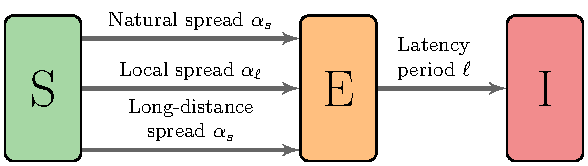
\includegraphics[height=.16\textwidth]{figs/SEI.pdf}
%%     \caption{Schematic of the SEI process.\label{fig:SEI}}
%% \end{figure}
%%
%% 
%% \paragraph{Susceptibility and infectiousness of a cell.} We have used
%% monthly production to determine the susceptiblity of a cell in state~$S$
%% and infectiousness of a cell in state~$I$. The suitability of a cell~$v$
%% for pest establishment at time~$t$ is denoted by~$\suitable(v,t)$. This
%% is~$1$ if production at~$t$ is non-zero and~$0$ otherwise.  For a cell in
%% state~$I$, the level of infestation in an infected cell~$v$ at time~$t$ is
%% denoted by~$\infest(v,t)$. It is modeled as a linear function of host
%% presence at time~$t$, for which we use the weighted sum of production
%% volume of tomato, eggplant, and potato in that cell
%% at time~$t$. The weights correspond to relative oviposition preference of
%% \tuta{} on the three hosts.
%% 
%%


%% For each region, we obtained the product rate by
%% normalizing quarterly production values with respect to maximum value among
%% these. We used production rate instead of production values since there are
%% several factors that determine a region's production: climate, vegetable
%% preference, demand, etc.  Therefore, it may not be meaningful to compare
%% production across regions.  
%% We conducted a linear regression with the
%% product rate as a dependent variable and precipitation and temperature and
%% elevation as independent variables.  To control elevation, we classified
%% the elevations into two groups, high and low, using $k$-means clustering
%% (SPSS~24.0). Due to the small sample size, we excluded the samples in the
%% high-elevation group and conducted a linear regression analysis for the
%% group of low elevation~($< 235$ masl). 

%% There is very little data
%% available for validation. Most of the data is qualitative, just providing
%% information on growing and harvesting months. The regression function was
%% applied to locations of different countries where this information is
%% available and visually compared.  More details of the methods, country
%% specific data and challenges in this regard are covered in
%% Section~\ref{S:sec:prod}. The infectiousness of cell~$v$ at
%% time~$t$,~$\infest(v,t)$ is the production at~$t$, while its
%% suitability,~$\epsilon(v,t)$ is~$0$ if~$\infest(v,t)=0$ and~$1$ otherwise.
%% on data availability. The first method was used if only seasonal
%% production is available for a region or country. In this case, we first
%% estimated seasonal production in each cell and then disaggregated it
%% to obtain monthly production. Here, due to unavailability of data for tomato and eggplant, we used SPAM's total
%% vegetable production as surrogate. To disaggregate into monthly production,
%% we studied the relationship between production, precipitation, and elevation.
%% For lowland areas, %(elevation less than ???) 
%% production is negatively
%% correlated with precipitation ($r<-0.75$).

%% \paragraph{Network structure.} The resulting network consists of~$8,010$
%% cells and~$109$ localities.  
%%
%%
%% \begin{table}[t]
%%     \caption{Model parameters and variables, their ranges and references.\label{tab:data}}
%%     \centering
%% 	\small
%%     \begin{tabular}{l p{4cm} p{3cm} p{5cm}}
%%     %{cp{.25\textwidth}p{.25\textwidth}lr}
%% 		\hline		
%% 		Parameter & Description & Range/values & Source \\
%% \hline		
%% \hline
%% $\mooreRange$ & Range of Moore neighborhood & 1,2,3 &
%% \cite{guimapi2016modeling}\\
%% $\ell$ & Latency period to transition from $E$ to $I$& 1,2,3 & \\
%% \hline
%% $\beta, \kappa$ & Gravity model parameters & 300--500,2 &
%% \cite{venkatramanan2017towards}\\
%% -- & Locality population threshold and radius & 250,000, 100kms &
%% population of cities~\cite{citypop} and reports\\
%% \hline
%% $\suitable$ & Suitability threshold & 0\\
%% $\infest$ & Infectivity of a cell based on amount of production & & Host
%% production (SPAM), host preference~\cite{sylla2018}, precipitation and
%% elevation \\
%% \hline
%% Scenarios & Seeding simulations: time and cells to infect & 4 cases:
%% Bangladesh (B1 and B2), Malaysia (M1) and Philippines (P1) & \tuta{} incidence
%% reports in Bangladesh, FAOSTAT for international trade and migration
%% reports.\\
%% Start month & & March, April, May & Based on incidence reports\\
%% \hline
%% $\asd$ & Short-distance spread scaling factor & 0--500\\
%% $\afm$ & Local human-mediated dispersal scaling factor & 0--500\\
%% $\ald$ & Long distance spread scaling factor & 0--500 \\
%% \hline
%% \end{tabular}
%% \end{table}
%%

%% In the first part of this section, we present results from the analysis of
%% the spread of \tuta{} in Bangladesh. We demonstrate how accounting for
%% different pathways affects the rate as well as pattern of spread. In the
%% second part, we focus on threat and possible spread in the rest of the
%% study region. The last part focuses on monitoring and control.
%%
%%
%% This section is organized as follows. We first describe the multi-pathway
%% model--our methodological contribution.  This is followed by our results in
%% the context of \tuta{} spread which are summarized as follows: (i)~We
%% identified possible routes by which \tuta{} can invade each country in the
%% region by analysis of current distribution of the pest and its.
%%
%% \paragraph{Assessing the role of each pathway in the spread of \tuta{} in
%% Bangladesh.} 
